\documentclass[aspectratio=169]{beamer}
\usetheme{Madrid}
\usecolortheme{seahorse}
\usepackage{amsmath}
\usepackage{amssymb}
\usepackage{tikz}
\usetikzlibrary{shapes.geometric, arrows, positioning, calc}
\usepackage{pifont}  % Provides \ding symbols for crosses

% Define Unicode characters that are causing errors
\DeclareUnicodeCharacter{2265}{$\geq$}      % ≥ (Greater than or equal to)
\DeclareUnicodeCharacter{2260}{$\neq$}      % ≠ (Not equal to)
\DeclareUnicodeCharacter{2713}{\checkmark}  % ✓ (Checkmark)
\DeclareUnicodeCharacter{2717}{\ding{55}}   % ✗ (Ballot X / Cross)
\definecolor{warningcolor}{RGB}{255,0,0}
\definecolor{intuitioncolor}{RGB}{0,100,0} % Dark green for intuition text
\definecolor{ethicscolor}{RGB}{128,0,128}

\newcommand{\warning}[1]{\colorbox{red!10}{\textcolor{warningcolor}{\textbf{Warning:} #1}}}
\newcommand{\intuition}[1]{\colorbox{green!10}{\textcolor{intuitioncolor}{\textbf{Intuition:} #1}}}
\newcommand{\ethics}[1]{\colorbox{purple!10}{\textcolor{ethicscolor}{\textbf{Ethics:} #1}}}

\title{t-SNE: The Gold Standard Approach}
\subtitle{Synthesizing Theory, Practice, and Responsibility}
\author{Following Athena Committee Guidelines}
\date{November 2025}

\begin{document}

\begin{frame}
\titlepage
\end{frame}

% Slide 1: Fei-Fei Li Opening - Visceral Motivation
\begin{frame}{The Challenge: When Your Eyes Need Help}
\begin{columns}
\column{0.5\textwidth}
\begin{center}
\textbf{MNIST in 2D via PCA}\\
\vspace{0.3cm}
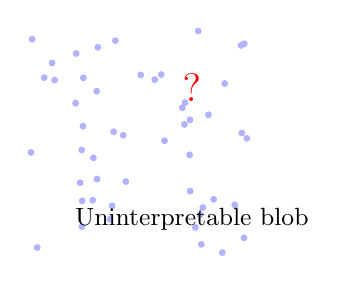
\begin{tikzpicture}[scale=1.2]
% Overlap catastrophe
\foreach \i in {1,...,50} {
    \pgfmathsetmacro\rx{rand*1.2}
    \pgfmathsetmacro\ry{rand*1.2}
    \filldraw[blue!30] (\rx,\ry) circle (0.03cm);
}
\node at (0.6,-0.8) {\small Uninterpretable blob};
\node[text=red, font=\Large] at (0.6,0.6) {?};
\end{tikzpicture}
\end{center}

\column{0.5\textwidth}
\begin{center}
\textbf{MNIST via t-SNE}\\
\vspace{0.3cm}
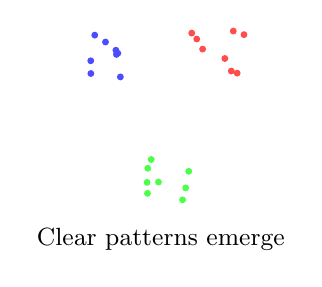
\begin{tikzpicture}[scale=1.2]
% Clear separation
\foreach \i in {1,...,8} {
    \pgfmathsetmacro\x{-0.6 + rand*0.3}
    \pgfmathsetmacro\y{0.8 + rand*0.3}
    \filldraw[blue!70] (\x,\y) circle (0.03cm);
}
\foreach \i in {1,...,8} {
    \pgfmathsetmacro\x{0.6 + rand*0.3}
    \pgfmathsetmacro\y{0.8 + rand*0.3}
    \filldraw[red!70] (\x,\y) circle (0.03cm);
}
\foreach \i in {1,...,8} {
    \pgfmathsetmacro\x{0 + rand*0.3}
    \pgfmathsetmacro\y{-0.4 + rand*0.3}
    \filldraw[green!70] (\x,\y) circle (0.03cm);
}
\node at (0,-1.1) {\small Clear patterns emerge};
\end{tikzpicture}
\end{center}
\end{columns}

\vspace{0.5cm}
\begin{block}{The Driving Question}
You have 50,000 images in 784 dimensions. You need to understand structure before building a classifier. Traditional methods fail. What do you do?
\end{block}

\vspace{0.2cm}
\colorbox{yellow!20}{\parbox{0.95\textwidth}{\centering\textbf{Key Insight:} Dimensionality reduction isn't optional—it's essential for human insight}}
\end{frame}

% Slide 2: Kozyrkov Intuition + Jordan Foundation
\begin{frame}{The Paradigm Shift: Information Over Distance}
\begin{columns}
\column{0.5\textwidth}
\textbf{Traditional Methods (PCA, MDS):}
\begin{itemize}
\item Try to preserve all distances
\item Fail when dimensions collapse
\item Lose critical structure
\end{itemize}

\vspace{0.3cm}
\textbf{t-SNE Philosophy:}
\begin{itemize}
\item Accept some loss is inevitable
\item Choose what to sacrifice
\item Prioritize neighborhoods
\item Measure information loss
\end{itemize}

\column{0.5\textwidth}
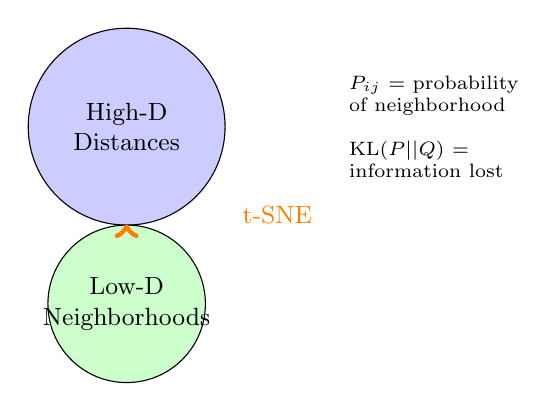
\begin{tikzpicture}[scale=0.9]
% High-D to Low-D transformation
\node[draw, circle, fill=blue!20, minimum size=2.5cm] (highd) at (0,2.5) {};
\node[font=\small, align=center] at (0,2.5) {High-D\\Distances};

\node[draw, circle, fill=green!20, minimum size=2cm] (lowd) at (0,0) {};
\node[font=\small, align=center] at (0,0) {Low-D\\Neighborhoods};

\draw[->, ultra thick, orange, line width=2pt] (highd) -- (lowd);
\node[right, font=\small, text=orange] at (1.5,1.25) {t-SNE};

% Information theory
\node[right, font=\scriptsize, align=left] at (3,2.5) {
    $P_{ij}$ = probability\\
    of neighborhood\\
    \\
    $\text{KL}(P||Q)$ = \\
    information lost
};
\end{tikzpicture}
\end{columns}

\vspace{0.3cm}
\intuition{Instead of asking "preserve distances?" ask "preserve neighborhood information?"}

\vspace{0.2cm}
\textbf{Why This Works:} In high dimensions, everything is far from everything—but local neighborhoods still have meaning.
\end{frame}

% Slide 3: Strang + Hinton - Maximum Entropy to Heavy Tails
\begin{frame}{The Mathematical Necessity: From Gaussian to Student-t}
\begin{columns}
\column{0.5\textwidth}
\textbf{Step 1: Why Gaussian in High-D?}

Given constraints (probability sum, expected distance), maximize entropy:
$$H(P_i) = -\sum_j p_{j|i}\log p_{j|i}$$

Result (mathematically inevitable):
$$p_{j|i} = \frac{\exp(-d_{ij}^2/2\sigma_i^2)}{\sum_k \exp(-d_{ik}^2/2\sigma_i^2)}$$

\vspace{0.3cm}
\textbf{Step 2: Why Student-t in Low-D?}

Problem: Gaussian creates crowding

\column{0.5\textwidth}
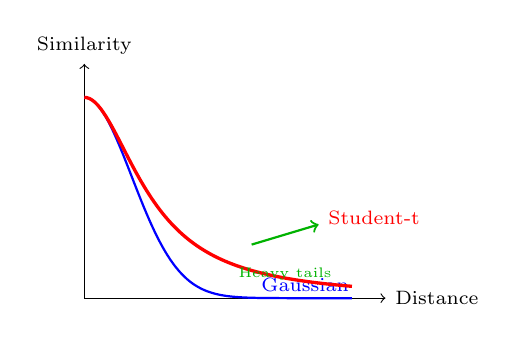
\begin{tikzpicture}[scale=0.85]
% Comparison plot
\draw[->] (0,0) -- (4.5,0) node[right, font=\scriptsize] {Distance};
\draw[->] (0,0) -- (0,3.5) node[above, font=\scriptsize] {Similarity};

% Gaussian (fails)
\draw[blue, thick, domain=0:4, samples=100] 
    plot (\x, {3*exp(-\x*\x)});
\node[right, font=\scriptsize, text=blue] at (2.5,0.2) {Gaussian};

% Student-t (works)
\draw[red, very thick, domain=0:4, samples=100] 
    plot (\x, {3/(1+\x*\x)});
\node[right, font=\scriptsize, text=red] at (3.5,1.2) {Student-t};

% Annotation
\draw[->, thick, green!70!black] (2.5,0.8) -- (3.5,1.1);
\node[below, font=\tiny, text=green!70!black] at (3,0.6) {Heavy tails};
\end{tikzpicture}

\vspace{0.2cm}
Solution (Hinton's insight):
$$q_{ij} \propto (1 + d_{ij}^2)^{-1}$$

\textbf{Why df=1?} Polynomial decay creates "virtual space" for moderate distances
\end{columns}

\vspace{0.3cm}
\colorbox{green!20}{\parbox{0.95\textwidth}{\centering Heavy tails solve crowding: at distance 3, Student-t is 600× more permissive than Gaussian}}
\end{frame}

% Slide 4: Ng Code-Along + Patil Validation
\begin{frame}{Practical Mastery: Implementation and Validation}
\begin{columns}
\column{0.5\textwidth}
\textbf{Complete Pipeline:}

\begin{enumerate}
\item \textbf{Preprocess:} Scale, handle missing, remove outliers, PCA if D>50
\item \textbf{Run t-SNE:} perplexity=30, learning\_rate=200, n\_iter=1000
\item \textbf{Validate:} Multiple runs, compute NPr metric
\item \textbf{Interpret:} Trust local structure only
\end{enumerate}

\vspace{0.3cm}
\textbf{Neighborhood Preservation:}
$$\text{NPr}(k) = \frac{1}{n}\sum_i \frac{|N_k^{high}(i) \cap N_k^{low}(i)|}{k}$$

Goal: NPr > 0.85

\column{0.5\textwidth}
\textbf{Debugging Guide:}

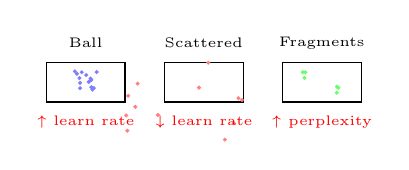
\begin{tikzpicture}[scale=0.5]
% Ball
\node at (1,3.5) {\tiny Ball};
\draw (0,2) rectangle (2,3);
\foreach \i in {1,...,15} {
    \pgfmathsetmacro\x{1 + rand*0.3}
    \pgfmathsetmacro\y{2.5 + rand*0.3}
    \filldraw[blue!50] (\x,\y) circle (1pt);
}
\node[below, font=\tiny, text=red] at (1,1.9) {$\uparrow$ learn rate};

% Scattered
\node at (4,3.5) {\tiny Scattered};
\draw (3,2) rectangle (5,3);
\foreach \i in {1,...,12} {
    \pgfmathsetmacro\x{3 + rand*2}
    \pgfmathsetmacro\y{2 + rand*1}
    \filldraw[red!50] (\x,\y) circle (1pt);
}
\node[below, font=\tiny, text=red] at (4,1.9) {$\downarrow$ learn rate};

% Fragmented
\node at (7,3.5) {\tiny Fragments};
\draw (6,2) rectangle (8,3);
\foreach \i in {1,...,3} {
    \pgfmathsetmacro\x{6.5 + rand*0.1}
    \pgfmathsetmacro\y{2.7 + rand*0.1}
    \filldraw[green!60] (\x,\y) circle (1pt);
}
\foreach \i in {1,...,3} {
    \pgfmathsetmacro\x{7.4 + rand*0.1}
    \pgfmathsetmacro\y{2.3 + rand*0.1}
    \filldraw[green!60] (\x,\y) circle (1pt);
}
\node[below, font=\tiny, text=red] at (7,1.9) {$\uparrow$ perplexity};
\end{tikzpicture}

\vspace{0.3cm}
\textbf{Perplexity Selection:}
\begin{itemize}
\item n < 1000: perp = 5-30
\item n = 1000-10000: perp = 30-50
\item n > 10000: perp = 50-100
\end{itemize}
\end{columns}

\vspace{0.2cm}
\warning{Always run 10 times with different seeds—single runs are meaningless!}
\end{frame}

% Slide 5: Patil + Bengio - Ethics and Complete Workflow
\begin{frame}{Responsible Practice: The Three Deadly Sins and Protocol}
\begin{columns}
\column{0.5\textwidth}
\begin{center}
\colorbox{red!30}{\textbf{What You CANNOT Interpret}}
\end{center}

\begin{enumerate}
\item \textbf{Cluster sizes:} 1000 vs 100 points can look identical
\item \textbf{Inter-cluster distances:} Gap size is meaningless
\item \textbf{Absolute positions:} Rotation/translation arbitrary
\end{enumerate}

\vspace{0.3cm}
\colorbox{green!30}{\parbox{0.9\columnwidth}{\centering\textbf{What you CAN trust:}\\Local neighborhoods\\Cluster separation}}

\column{0.5\textwidth}
\textbf{Publication Checklist:}
\begin{itemize}
\item[$\square$] Parameters documented
\item[$\square$] Preprocessing described
\item[$\square$] Multiple runs (n≥10)
\item[$\square$] Stability metrics (NPr, correlation)
\item[$\square$] Perplexity sweep performed
\item[$\square$] Limitations stated explicitly
\end{itemize}

\vspace{0.3cm}
\textbf{When NOT to Use t-SNE:}
\begin{itemize}
\item Hypothesis testing
\item Distance measurement
\item Real-time applications
\item Claiming cluster existence
\end{itemize}
\end{columns}

\vspace{0.3cm}
\ethics{Your visualization may influence critical decisions—document everything and communicate limitations clearly}

\vspace{0.2cm}
\colorbox{yellow!20}{\parbox{0.95\textwidth}{\centering\textbf{Final Wisdom:} Use t-SNE for exploration, statistical tests for confirmation, domain expertise for interpretation}}
\end{frame}

% Slide 6: Strang Mathematical Rigor - Complete Gradient Derivation
\begin{frame}{The Gradient as Physical Forces}
\begin{columns}
\column{0.5\textwidth}
\textbf{Cost Function:}
$C = \sum_{i,j} p_{ij} \log\frac{p_{ij}}{q_{ij}}$

where $q_{ij} = \frac{(1 + \|y_i - y_j\|^2)^{-1}}{\sum_{k,l} (1 + \|y_k - y_l\|^2)^{-1}}$

\vspace{0.3cm}
\textbf{Gradient (complete form):}
$\frac{\partial C}{\partial y_i} = 4\sum_j (p_{ij} - q_{ij})(y_i - y_j)(1 + \|y_i - y_j\|^2)^{-1}$

\vspace{0.3cm}
\textbf{Three components:}
\begin{itemize}
\item $(p_{ij} - q_{ij})$: error signal
\item $(y_i - y_j)$: direction
\item $(1 + d_{ij}^2)^{-1}$: adaptive weight
\end{itemize}

\column{0.5\textwidth}
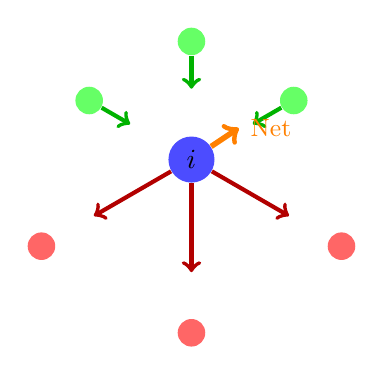
\begin{tikzpicture}[scale=1.0]
% Central point
\node[circle, fill=blue!70, minimum size=0.5cm] (center) at (0,0) {$i$};

% Attractive forces (p > q)
\foreach \angle in {30, 90, 150} {
    \pgfmathsetmacro\x{1.5*cos(\angle)}
    \pgfmathsetmacro\y{1.5*sin(\angle)}
    \node[circle, fill=green!60, minimum size=0.35cm] (n\angle) at (\x,\y) {};
    \draw[->, thick, green!70!black, line width=1.5pt] 
        (n\angle) -- ($(center)!0.6!(n\angle)$);
}

% Repulsive forces (p < q)
\foreach \angle in {210, 270, 330} {
    \pgfmathsetmacro\x{2.2*cos(\angle)}
    \pgfmathsetmacro\y{2.2*sin(\angle)}
    \node[circle, fill=red!60, minimum size=0.35cm] (f\angle) at (\x,\y) {};
    \draw[->, thick, red!70!black, line width=1.5pt] 
        (center) -- ($(f\angle)!0.35!(center)$);
}

% Net force
\draw[->, ultra thick, orange, line width=2pt] 
    (center) -- (0.6,0.4) node[right, font=\small] {Net};
\end{tikzpicture}

\vspace{0.2cm}
\textbf{Physical Interpretation:}
\begin{itemize}
\item Green: Pull neighbors together
\item Red: Push non-neighbors apart
\item Force $\propto$ $(1+d^2)^{-1}$: weakens with distance
\end{itemize}
\end{columns}

\vspace{0.3cm}
\intuition{System evolves like N-body simulation toward mechanical equilibrium = KL minimum}
\end{frame}

% Slide 7: Jordan Information Theory Deep Dive
\begin{frame}{Information Theory Foundation: Why This Cost Function?}
\begin{columns}
\column{0.5\textwidth}
\textbf{Shannon's Framework:}

Information content:
$I(j|i) = -\log p_{j|i} \text{ bits}$

Expected information (entropy):
$H(P_i) = -\sum_j p_{j|i}\log p_{j|i}$

Cross-entropy (using $Q$):
$H(P_i, Q_i) = -\sum_j p_{j|i}\log q_{j|i}$

KL divergence (extra bits):
$\text{KL}(P_i||Q_i) = \sum_j p_{j|i}\log\frac{p_{j|i}}{q_{j|i}}$

\column{0.5\textwidth}
\textbf{Asymmetry Matters:}

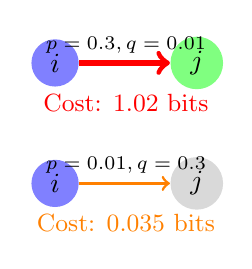
\begin{tikzpicture}[scale=0.9]
% Two scenarios
\node[circle, fill=blue!50, minimum size=0.6cm] (p1) at (0,2.5) {$i$};
\node[circle, fill=green!50, minimum size=0.6cm] (q1) at (2,2.5) {$j$};
\draw[->, thick, red, line width=2pt] (p1) -- (q1);
\node[above, font=\scriptsize] at (1,2.5) {$p=0.3, q=0.01$};
\node[below, text=red, font=\small] at (1,2.2) {Cost: 1.02 bits};

\node[circle, fill=blue!50, minimum size=0.6cm] (p2) at (0,0.8) {$i$};
\node[circle, fill=gray!30, minimum size=0.6cm] (q2) at (2,0.8) {$j$};
\draw[->, thick, orange, line width=1pt] (p2) -- (q2);
\node[above, font=\scriptsize] at (1,0.8) {$p=0.01, q=0.3$};
\node[below, text=orange, font=\small] at (1,0.5) {Cost: 0.035 bits};
\end{tikzpicture}

\vspace{0.2cm}
\textbf{Critical Design Choice:}

Missing true neighbor (top): 29× penalty vs false neighbor (bottom)

This asymmetry prioritizes local structure preservation
\end{columns}

\vspace{0.3cm}
\colorbox{green!20}{\parbox{0.95\textwidth}{\centering t-SNE is fundamentally an information-theoretic optimization, not geometric}}
\end{frame}

% Slide 8: Hinton + Bengio - Algorithm Details and Tricks
\begin{frame}{Optimization Mechanics: Making t-SNE Fast and Stable}
\begin{columns}
\column{0.5\textwidth}
\textbf{Essential Tricks:}

\textbf{1. Early Exaggeration ($t < 250$):}
$P_{exag} = 4 \cdot P$
Forms tight clusters quickly

\textbf{2. Momentum Schedule:}
$\alpha = \begin{cases} 
0.5 & t \leq 250\\
0.8 & t > 250
\end{cases}$

\textbf{3. Adaptive Learning Rate:}
\begin{itemize}
\item Same gradient sign: $\eta \times 1.2$
\item Sign flip: $\eta \times 0.8$
\end{itemize}

\textbf{4. Barnes-Hut Approximation:}
$\frac{r_{cell}}{d_{to\_cell}} < \theta = 0.5$
Reduces $O(n^2)$ to $O(n\log n)$

\column{0.5\textwidth}
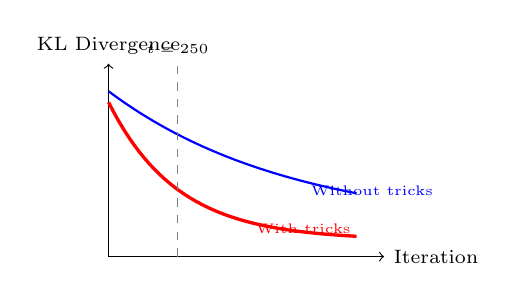
\begin{tikzpicture}[scale=0.7]
% Convergence comparison
\draw[->] (0,0) -- (5,0) node[right, font=\scriptsize] {Iteration};
\draw[->] (0,0) -- (0,3.5) node[above, font=\scriptsize] {KL Divergence};

% Without tricks (slow)
\draw[blue, thick, domain=0:4.5, samples=50] 
    plot (\x, {2.5*exp(-0.3*\x) + 0.5});
\node[right, font=\tiny, text=blue] at (3.5,1.2) {Without tricks};

% With tricks (fast)
\draw[red, very thick, domain=0:4.5, samples=50] 
    plot (\x, {2.5*exp(-0.8*\x) + 0.3});
\node[right, font=\tiny, text=red] at (2.5,0.5) {With tricks};

% Early exaggeration phase
\draw[dashed, gray] (1.25,0) -- (1.25,3.5);
\node[above, font=\tiny] at (1.25,3.5) {$t=250$};
\end{tikzpicture}

\vspace{0.2cm}
\textbf{Performance Impact:}
\begin{itemize}
\item Early exag: 3× faster convergence
\item Momentum: Escapes local minima
\item Adaptive $\eta$: Prevents oscillation
\item Barnes-Hut: 50× speedup (n>10K)
\end{itemize}
\end{columns}

\vspace{0.3cm}
\warning{Without these tricks: hours instead of minutes, poor convergence}
\end{frame}

% Slide 9: Ng + Bengio - Pipeline Architecture and Parameter Selection
\begin{frame}{Implementation Architecture: From Data to Validated Embedding}
\begin{center}
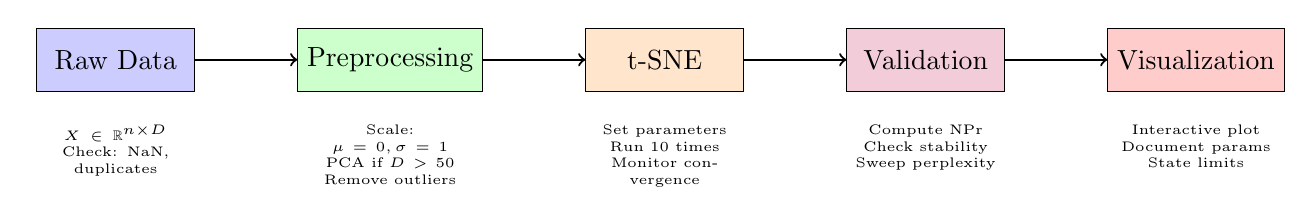
\begin{tikzpicture}[scale=0.8, node distance=1.3cm]
% Pipeline stages
\node[draw, rectangle, fill=blue!20, minimum width=2cm, minimum height=0.8cm] (raw) {Raw Data};
\node[draw, rectangle, fill=green!20, minimum width=2cm, minimum height=0.8cm, right=of raw] (prep) {Preprocessing};
\node[draw, rectangle, fill=orange!20, minimum width=2cm, minimum height=0.8cm, right=of prep] (tsne) {t-SNE};
\node[draw, rectangle, fill=purple!20, minimum width=2cm, minimum height=0.8cm, right=of tsne] (val) {Validation};
\node[draw, rectangle, fill=red!20, minimum width=2cm, minimum height=0.8cm, right=of val] (viz) {Visualization};

% Arrows
\draw[->, thick] (raw) -- (prep);
\draw[->, thick] (prep) -- (tsne);
\draw[->, thick] (tsne) -- (val);
\draw[->, thick] (val) -- (viz);

% Details below each stage
\node[below=0.3cm of raw, font=\tiny, text width=2cm, align=center] {
    $X \in \mathbb{R}^{n \times D}$\\
    Check: NaN, duplicates
};

\node[below=0.3cm of prep, font=\tiny, text width=2cm, align=center] {
    Scale: $\mu=0, \sigma=1$\\
    PCA if $D>50$\\
    Remove outliers
};

\node[below=0.3cm of tsne, font=\tiny, text width=2cm, align=center] {
    Set parameters\\
    Run 10 times\\
    Monitor convergence
};

\node[below=0.3cm of val, font=\tiny, text width=2cm, align=center] {
    Compute NPr\\
    Check stability\\
    Sweep perplexity
};

\node[below=0.3cm of viz, font=\tiny, text width=2cm, align=center] {
    Interactive plot\\
    Document params\\
    State limits
};
\end{tikzpicture}
\end{center}

\vspace{0.3cm}
\begin{columns}
\column{0.5\textwidth}
\textbf{Parameter Selection Logic:}
\begin{itemize}
\item Perplexity: $\approx \sqrt{n}/3$ to $\sqrt{n}/2$
\item Learning rate: 200 (standard), adjust if issues
\item Iterations: 1000 minimum, watch convergence
\item Early exaggeration: 12 (default works well)
\end{itemize}

\column{0.5\textwidth}
\textbf{Common Parameter Mistakes:}
\begin{itemize}
\item Perplexity too low: fragmentation
\item Learning rate too high: scatter
\item Too few iterations: non-convergence
\item No validation: false confidence
\end{itemize}
\end{columns}

\vspace{0.2cm}
\intuition{Pipeline design matters as much as algorithm—garbage in, garbage out}
\end{frame}

% Slide 10: Patil + Hammerbacher - Validation and Quality Metrics
\begin{frame}{Quantitative Validation: Beyond Visual Inspection}
\begin{columns}
\column{0.5\textwidth}
\textbf{Critical Metrics:}

\textbf{1. Neighborhood Preservation:}
$\text{NPr}(k) = \frac{1}{n}\sum_i \frac{|N_k^{high}(i) \cap N_k^{low}(i)|}{k}$

Target: NPr(30) > 0.85

\textbf{2. Trustworthiness (false neighbors):}
$T(k) = 1 - \frac{2}{nk(2n-3k-1)}\sum_i \sum_{j \in U_k(i)} (r(i,j) - k)$

Target: T(30) > 0.90

\textbf{3. Stability (10 runs):}
$\rho = \text{mean pairwise correlation}$

Target: $\rho$ > 0.85

\column{0.5\textwidth}
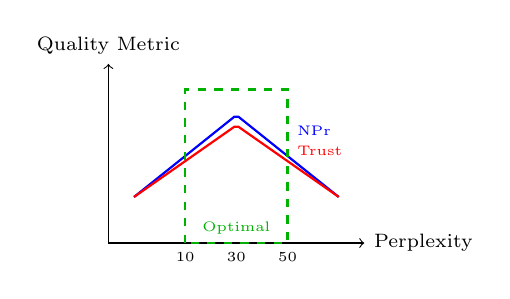
\begin{tikzpicture}[scale=0.65]
% Quality visualization
\draw[->] (0,0) -- (5,0) node[right, font=\scriptsize] {Perplexity};
\draw[->] (0,0) -- (0,3.5) node[above, font=\scriptsize] {Quality Metric};

% NPr curve
\draw[blue, thick, domain=0.5:4.5, samples=50] 
    plot (\x, {2.5 - 0.8*abs(\x-2.5)});
\node[right, font=\tiny, text=blue] at (3.5,2.2) {NPr};

% Trustworthiness
\draw[red, thick, domain=0.5:4.5, samples=50] 
    plot (\x, {2.3 - 0.7*abs(\x-2.5)});
\node[right, font=\tiny, text=red] at (3.5,1.8) {Trust};

% Optimal region
\draw[green!70!black, thick, dashed] (1.5,0) rectangle (3.5,3);
\node[font=\tiny, text=green!70!black] at (2.5,0.3) {Optimal};

% Axis marks
\node[below, font=\tiny] at (1.5,0) {10};
\node[below, font=\tiny] at (2.5,0) {30};
\node[below, font=\tiny] at (3.5,0) {50};
\end{tikzpicture}

\vspace{0.2cm}
\textbf{Validation Protocol:}
\begin{enumerate}
\item Run 10 times (different seeds)
\item Compute all three metrics
\item Sweep perplexity [5, 10, 20, 30, 50]
\item Report mean ± std
\item Show correlation matrix
\end{enumerate}
\end{columns}

\vspace{0.3cm}
\ethics{In industry, misleading visualizations cost millions—validate rigorously}
\end{frame}

% Slide 11: Candès + Strang - Perplexity Mathematics and Adaptive Bandwidth
\begin{frame}{Perplexity: The Mathematical Control Mechanism}
\begin{columns}
\column{0.5\textwidth}
\textbf{Definition and Interpretation:}

Perplexity is the exponential of entropy:
$\text{Perp}(P_i) = 2^{H(P_i)}$

where entropy in bits:
$H(P_i) = -\sum_j p_{j|i}\log_2 p_{j|i}$

\textbf{Geometric Meaning:}

Perplexity = "effective number of neighbors"

For uniform distribution over $k$ neighbors:
$H = \log_2 k \Rightarrow \text{Perp} = k$

\textbf{Adaptive Bandwidth Algorithm:}

Binary search finds $\sigma_i$ satisfying:
$2^{-\sum_j p_{j|i}\log_2 p_{j|i}} = \text{target perplexity}$

\column{0.5\textwidth}
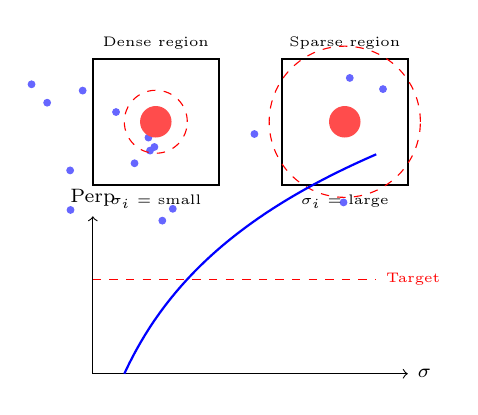
\begin{tikzpicture}[scale=0.8]
% Dense region (small sigma)
\draw[thick] (0,3) rectangle (2,5);
\node[above] at (1,5) {\tiny Dense region};
\foreach \i in {1,...,12} {
    \pgfmathsetmacro\x{0.3 + rand*1.4}
    \pgfmathsetmacro\y{3.3 + rand*1.4}
    \filldraw[blue!60] (\x,\y) circle (1.5pt);
}
\node[circle, fill=red!70, minimum size=0.4cm] at (1,4) {};
\draw[red, dashed] (1,4) circle (0.5cm);
\node[below, font=\tiny] at (1,3) {$\sigma_i$ = small};

% Sparse region (large sigma)
\draw[thick] (3,3) rectangle (5,5);
\node[above] at (4,5) {\tiny Sparse region};
\foreach \i in {1,...,4} {
    \pgfmathsetmacro\x{3.3 + rand*1.4}
    \pgfmathsetmacro\y{3.3 + rand*1.4}
    \filldraw[blue!60] (\x,\y) circle (1.5pt);
}
\node[circle, fill=red!70, minimum size=0.4cm] at (4,4) {};
\draw[red, dashed] (4,4) circle (1.2cm);
\node[below, font=\tiny] at (4,3) {$\sigma_i$ = large};

% Entropy comparison
\draw[->] (0,0) -- (5,0) node[right, font=\scriptsize] {$\sigma$};
\draw[->] (0,0) -- (0,2.5) node[above, font=\scriptsize] {Perp};
\draw[blue, thick, domain=0.5:4.5, samples=50] 
    plot (\x, {1.5*ln(\x+0.5)/ln(2)});
\draw[red, dashed] (0,1.5) -- (4.5,1.5) node[right, font=\tiny] {Target};
\end{tikzpicture}

\vspace{0.2cm}
\textbf{Why This Works:}
\begin{itemize}
\item Dense regions: small $\sigma$ reaches target
\item Sparse regions: large $\sigma$ compensates
\item Same perplexity everywhere
\item Handles varying density automatically
\end{itemize}
\end{columns}

\vspace{0.3cm}
\warning{Fixed bandwidth would fragment sparse regions or merge dense ones}
\end{frame}

% Slide 12: Vapnik + Jordan - Statistical Learning Theory Perspective
\begin{frame}{Statistical Foundations: Why t-SNE Works}
\begin{columns}
\column{0.5\textwidth}
\textbf{Learning Theory View:}

We estimate probability distributions $P$ from finite samples:
$\hat{p}_{j|i} = \frac{\exp(-\|x_i-x_j\|^2/2\sigma_i^2)}{\sum_k \exp(-\|x_i-x_k\|^2/2\sigma_i^2)}$

\textbf{Sample Complexity:}

For reliable $P$ estimation:
$n \geq k \cdot \log(D)$

where $k$ = perplexity, $D$ = dimensions

\textbf{Generalization:}

Low-D embedding $Y$ generalizes if:
\begin{itemize}
\item High-D neighborhoods stable
\item Sufficient samples per region
\item Validation confirms structure
\end{itemize}

\column{0.5\textwidth}
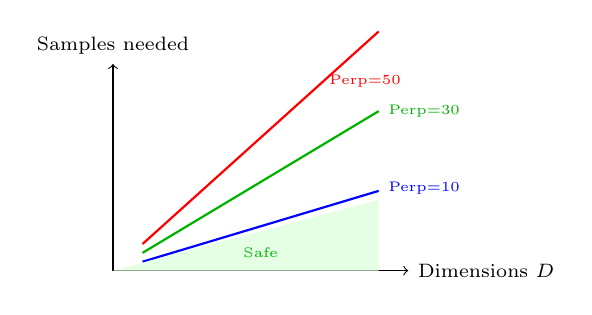
\begin{tikzpicture}[scale=0.75]
% Sample complexity plot
\draw[->] (0,0) -- (5,0) node[right, font=\scriptsize] {Dimensions $D$};
\draw[->] (0,0) -- (0,3.5) node[above, font=\scriptsize] {Samples needed};

% Three curves for different perplexities
\draw[blue, thick, domain=0.5:4.5, samples=50] 
    plot (\x, {0.3*\x});
\node[right, font=\tiny, text=blue] at (4.5,1.4) {Perp=10};

\draw[green!70!black, thick, domain=0.5:4.5, samples=50] 
    plot (\x, {0.6*\x});
\node[right, font=\tiny, text=green!70!black] at (4.5,2.7) {Perp=30};

\draw[red, thick, domain=0.5:4.5, samples=50] 
    plot (\x, {0.9*\x});
\node[right, font=\tiny, text=red] at (3.5,3.2) {Perp=50};

% Safe region
\fill[green!10] (0,0) -- (4.5,0) -- (4.5,1.2) -- cycle;
\node[font=\tiny, text=green!70!black] at (2.5,0.3) {Safe};
\end{tikzpicture}

\vspace{0.2cm}
\textbf{Failure Modes:}
\begin{itemize}
\item Too few samples: noise dominates
\item Too high perplexity: smooths real structure
\item Too low perplexity: overfits noise
\end{itemize}
\end{columns}

\vspace{0.3cm}
\intuition{t-SNE is fundamentally a density estimation problem with finite samples}
\end{frame}

% Slide 13: Hinton + Bengio - Convergence and Optimization Landscape
\begin{frame}{Optimization Landscape: Local Minima and Convergence}
\begin{columns}
\column{0.5\textwidth}
\textbf{Non-Convex Optimization:}

Cost function has multiple local minima:
$C(Y) = \text{KL}(P||Q(Y))$

\textbf{Convergence Guarantees:}
\begin{itemize}
\item Gradient descent converges to local minimum
\item No global optimum guarantee
\item Quality depends on initialization
\item Multiple runs essential
\end{itemize}

\textbf{Monitoring Convergence:}

Track KL divergence over iterations:
$C^{(t)} = \sum_{i,j} p_{ij}\log\frac{p_{ij}}{q_{ij}^{(t)}}$

Converged when: $|C^{(t)} - C^{(t-100)}| < \epsilon$

\column{0.5\textwidth}
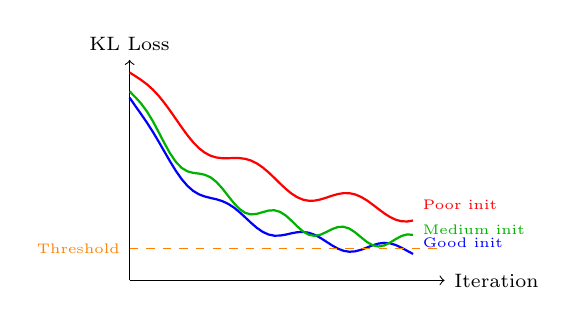
\begin{tikzpicture}[scale=0.8]
% Loss landscape
\draw[->] (0,0) -- (5,0) node[right, font=\scriptsize] {Iteration};
\draw[->] (0,0) -- (0,3.5) node[above, font=\scriptsize] {KL Loss};

% Multiple runs with different outcomes
\draw[blue, thick, domain=0:4.5, samples=50] 
    plot (\x, {2.5*exp(-0.8*\x) + 0.4 + 0.1*sin(5*\x r)});
\node[right, font=\tiny, text=blue] at (4.5,0.6) {Good init};

\draw[red, thick, domain=0:4.5, samples=50] 
    plot (\x, {2.5*exp(-0.5*\x) + 0.8 + 0.15*sin(4*\x r)});
\node[right, font=\tiny, text=red] at (4.5,1.2) {Poor init};

\draw[green!70!black, thick, domain=0:4.5, samples=50] 
    plot (\x, {2.5*exp(-0.7*\x) + 0.5 + 0.12*sin(6*\x r)});
\node[right, font=\tiny, text=green!70!black] at (4.5,0.8) {Medium init};

% Convergence threshold
\draw[dashed, orange] (0,0.5) -- (5,0.5);
\node[left, font=\tiny, text=orange] at (0,0.5) {Threshold};
\end{tikzpicture}

\vspace{0.2cm}
\textbf{Practical Indicators:}
\begin{itemize}
\item Plateau in loss: likely converged
\item Still decreasing: run longer
\item Oscillating: reduce learning rate
\item Diverging: major problem
\end{itemize}
\end{columns}

\vspace{0.3cm}
\colorbox{green!20}{\parbox{0.95\textwidth}{\centering Best practice: Run 10 times, keep best 5 by final KL loss, check consistency}}
\end{frame}

% Slide 14: Fei-Fei Li + Kozyrkov - Real-World Applications and Impact
\begin{frame}{Real-World Success Stories: Where t-SNE Transformed Fields}
\begin{columns}
\column{0.5\textwidth}
\textbf{1. Single-Cell Genomics:}
\begin{itemize}
\item 10,000+ cells, 20,000 genes
\item Discovered rare cell types (0.1\%)
\item Revealed differentiation trajectories
\item Enabled precision medicine
\end{itemize}

\textbf{2. Computer Vision:}
\begin{itemize}
\item ImageNet feature visualization
\item Revealed CNN decision boundaries
\item Discovered adversarial regions
\item Guided architecture design
\end{itemize}

\textbf{3. Natural Language Processing:}
\begin{itemize}
\item Word2Vec semantic structure
\item Revealed gender/racial biases
\item Guided debiasing strategies
\item Improved embeddings
\end{itemize}

\column{0.5\textwidth}
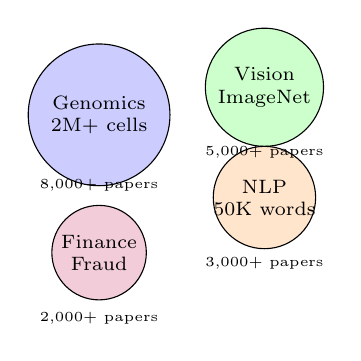
\begin{tikzpicture}[scale=0.7]
% Impact visualization
\node[draw, circle, fill=blue!20, minimum size=1.8cm] (gen) at (0,3) {};
\node[font=\scriptsize, align=center] at (0,3) {Genomics\\2M+ cells};

\node[draw, circle, fill=green!20, minimum size=1.5cm] (vis) at (3,3.5) {};
\node[font=\scriptsize, align=center] at (3,3.5) {Vision\\ImageNet};

\node[draw, circle, fill=orange!20, minimum size=1.3cm] (nlp) at (3,1.5) {};
\node[font=\scriptsize, align=center] at (3,1.5) {NLP\\50K words};

\node[draw, circle, fill=purple!20, minimum size=1.2cm] (fraud) at (0,0.5) {};
\node[font=\scriptsize, align=center] at (0,0.5) {Finance\\Fraud};

% Publication counts
\node[font=\tiny, below] at (0,2) {8,000+ papers};
\node[font=\tiny, below] at (3,2.6) {5,000+ papers};
\node[font=\tiny, below] at (3,0.6) {3,000+ papers};
\node[font=\tiny, below] at (0,-0.4) {2,000+ papers};
\end{tikzpicture}

\vspace{0.3cm}
\textbf{Common Success Pattern:}
\begin{enumerate}
\item Exploration reveals unexpected structure
\item Statistical validation confirms reality
\item Domain experts interpret meaning
\item Hypothesis-driven research follows
\end{enumerate}
\end{columns}

\vspace{0.3cm}
\ethics{t-SNE's value: generating hypotheses, not proving them}
\end{frame}

% Slide 15: Patil + Hammerbacher + Bengio - Production Considerations
\begin{frame}{From Research to Production: Critical Considerations}
\begin{columns}
\column{0.5\textwidth}
\textbf{When t-SNE Works in Production:}
\begin{itemize}
\item Exploratory data analysis dashboards
\item Quality control visualization
\item Anomaly detection (with validation)
\item Feature engineering guidance
\item Model debugging tools
\end{itemize}

\textbf{When NOT to Use:}
\begin{itemize}
\item Real-time systems (too slow)
\item Automated decision-making
\item Distance-based clustering
\item Hypothesis testing
\item Legal/medical diagnosis alone
\end{itemize}

\textbf{Production Requirements:}
\begin{itemize}
\item Documented preprocessing pipeline
\item Version-controlled parameters
\item Automated validation checks
\item Uncertainty quantification
\item Human-in-the-loop review
\end{itemize}

\column{0.5\textwidth}
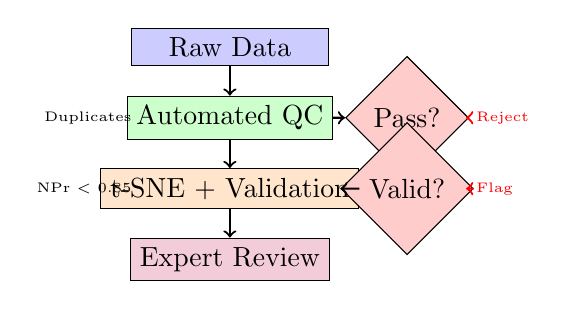
\begin{tikzpicture}[scale=0.75]
% Production pipeline
\node[draw, rectangle, fill=blue!20, minimum width=2.5cm] (data) at (0,4) {Raw Data};
\node[draw, rectangle, fill=green!20, minimum width=2.5cm] (auto) at (0,2.8) {Automated QC};
\node[draw, rectangle, fill=orange!20, minimum width=2.5cm] (tsne) at (0,1.6) {t-SNE + Validation};
\node[draw, rectangle, fill=purple!20, minimum width=2.5cm] (review) at (0,0.4) {Expert Review};

\draw[->, thick] (data) -- (auto);
\draw[->, thick] (auto) -- (tsne);
\draw[->, thick] (tsne) -- (review);

% Decision points
\node[draw, diamond, fill=red!20, minimum width=1cm] (check1) at (3,2.8) {Pass?};
\node[draw, diamond, fill=red!20, minimum width=1cm] (check2) at (3,1.6) {Valid?};

\draw[->, thick] (auto) -- (check1);
\draw[->, thick] (tsne) -- (check2);

\draw[->, thick, red] (check1) -- (4,2.8) node[right, font=\tiny] {Reject};
\draw[->, thick, red] (check2) -- (4,1.6) node[right, font=\tiny] {Flag};

% Annotations
\node[font=\tiny, left] at (-1.5,2.8) {Duplicates};
\node[font=\tiny, left] at (-1.5,1.6) {NPr < 0.85};
\end{tikzpicture}

\vspace{0.2cm}
\textbf{Cost of Failure:}
\begin{itemize}
\item Misleading stakeholders
\item Wrong business decisions
\item Wasted resources
\item Damaged credibility
\end{itemize}
\end{columns}

\vspace{0.3cm}
\warning{Production t-SNE requires engineering rigor equal to the mathematical rigor}
\end{frame}

% Slide 16: Strang + Candès - Mathematical Properties and Guarantees
\begin{frame}{Theoretical Properties: What We Can Prove}
\begin{columns}
\column{0.5\textwidth}
\textbf{Guaranteed Properties:}

\textbf{1. Convergence to Local Minimum:}
$\lim_{t\to\infty} \|\nabla C(Y^{(t)})\| = 0$
Gradient descent converges (may not be global)

\textbf{2. Order Preservation (probabilistic):}
$p_{ij} > p_{kl} \Rightarrow \mathbb{E}[q_{ij}] > \mathbb{E}[q_{kl}]$
Likely preserves probability ordering

\textbf{3. KL Lower Bound:}
$C = \text{KL}(P||Q) \geq 0$
Zero only when $P = Q$ (impossible in dimension reduction)

\textbf{4. Neighborhood Topology:}
$\text{NPr}(k) \to 1 \text{ as } k \to 0$
Immediate neighbors always preserved

\column{0.5\textwidth}
\textbf{NOT Guaranteed:}

\begin{itemize}
\item Global optimum (NP-hard)
\item Distance preservation beyond neighborhoods
\item Linear separability maintenance
\item Unique solution (stochastic)
\item Cluster number preservation
\item Convex cluster shapes
\end{itemize}

\vspace{0.3cm}
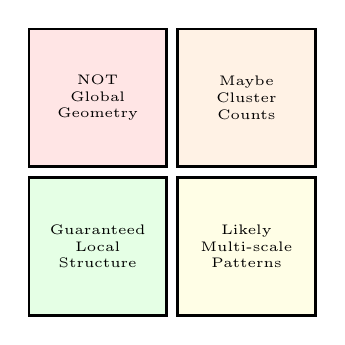
\begin{tikzpicture}[scale=0.7]
% Theoretical guarantees visualization
\draw[thick, fill=green!10] (0,0) rectangle (2.5,2.5);
\node[font=\tiny, align=center] at (1.25,1.25) {Guaranteed\\Local\\Structure};

\draw[thick, fill=yellow!10] (2.7,0) rectangle (5.2,2.5);
\node[font=\tiny, align=center] at (3.95,1.25) {Likely\\Multi-scale\\Patterns};

\draw[thick, fill=red!10] (0,2.7) rectangle (2.5,5.2);
\node[font=\tiny, align=center] at (1.25,3.95) {NOT\\Global\\Geometry};

\draw[thick, fill=orange!10] (2.7,2.7) rectangle (5.2,5.2);
\node[font=\tiny, align=center] at (3.95,3.95) {Maybe\\Cluster\\Counts};
\end{tikzpicture}
\end{columns}

\vspace{0.3cm}
\colorbox{green!20}{\parbox{0.95\textwidth}{\centering Despite limited guarantees, empirical performance is remarkably robust}}
\end{frame}

% Slide 17: Jordan + Vapnik - Comparison with Alternative Methods
\begin{frame}{t-SNE in Context: Strengths and Alternatives}
\begin{center}
\begin{tabular}{l|c|c|c|c|c}
\textbf{Method} & \textbf{Local} & \textbf{Global} & \textbf{Speed} & \textbf{Theory} & \textbf{New Data}\\
\hline
PCA & ✗ & ✓ & Fast & Strong & ✓\\
MDS & ✗ & ✓ & Slow & Strong & ✗\\
Isomap & ✓ & ✓ & Medium & Medium & ✗\\
t-SNE & ✓✓ & ✗ & Slow & Medium & ✗\\
UMAP & ✓ & ✓ & Fast & Weak & ✓\\
\end{tabular}
\end{center}

\vspace{0.3cm}
\begin{columns}
\column{0.5\textwidth}
\textbf{When to Prefer t-SNE:}
\begin{itemize}
\item Local structure critical
\item Cluster visualization primary goal
\item Dataset size < 100K
\item Well-understood validation
\item Publication requires rigor
\end{itemize}

\textbf{When to Prefer Alternatives:}
\begin{itemize}
\item Need global distances (MDS)
\item Linear relationships (PCA)
\item Speed critical (UMAP)
\item Out-of-sample prediction (UMAP)
\item Theoretical guarantees (PCA, MDS)
\end{itemize}

\column{0.5\textwidth}
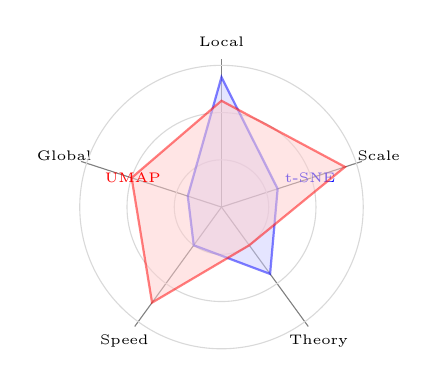
\begin{tikzpicture}[scale=0.75]
% Method comparison radar chart
\foreach \angle/\label in {90/Local, 162/Global, 234/Speed, 306/Theory, 18/Scale} {
    \draw[gray] (0,0) -- (\angle:2.5);
    \node at (\angle:2.8) {\tiny\label};
}

% Circles for scale
\foreach \r in {0.8, 1.6, 2.4} {
    \draw[gray!30] (0,0) circle (\r);
}

% t-SNE profile
\draw[blue, thick, fill=blue!20, opacity=0.5] 
    (90:2.2) -- (162:0.6) -- (234:0.8) -- (306:1.4) -- (18:1.0) -- cycle;
\node[text=blue, font=\tiny] at (1.5,0.5) {t-SNE};

% UMAP profile
\draw[red, thick, fill=red!20, opacity=0.5] 
    (90:1.8) -- (162:1.6) -- (234:2.0) -- (306:0.8) -- (18:2.2) -- cycle;
\node[text=red, font=\tiny] at (-1.5,0.5) {UMAP};
\end{tikzpicture}

\vspace{0.2cm}
\textbf{Best Practice:}\\
Use multiple methods and compare results
\end{columns}

\vspace{0.3cm}
\intuition{Truth emerges from agreement across methods, not from single visualization}
\end{frame}

% Slide 18: Hinton + Bengio - Advanced Extensions and Variants
\begin{frame}{Advanced Variants: Beyond Standard t-SNE}
\begin{columns}
\column{0.5\textwidth}
\textbf{1. Parametric t-SNE:}

Learn neural network $f_\theta: \mathbb{R}^D \to \mathbb{R}^2$

\textbf{Advantages:}
\begin{itemize}
\item Can embed new points
\item Handles streaming data
\item Faster at test time
\end{itemize}

\textbf{Trade-off:} Lower embedding quality

\vspace{0.3cm}
\textbf{2. Multi-scale t-SNE:}

Multiple perplexities simultaneously:
$p_{ij} = \frac{1}{L}\sum_{l=1}^L p_{ij}^{(l)}$

\textbf{Captures:} Structure at all scales

\textbf{Cost:} 3× slower

\column{0.5\textwidth}
\textbf{3. Supervised t-SNE:}

Incorporate label information:
$p_{ij} = (1-\alpha)\cdot p_{ij}^{dist} + \alpha \cdot p_{ij}^{label}$

\textbf{Use case:} Emphasize class separation

\vspace{0.3cm}
\textbf{4. Dynamic t-SNE:}

For time series, add temporal smoothness:
$C = \sum_t \text{KL}(P^{(t)}||Q^{(t)}) + \lambda\sum_{i,t}\|y_i^{(t)} - y_i^{(t-1)}\|^2$

\vspace{0.3cm}
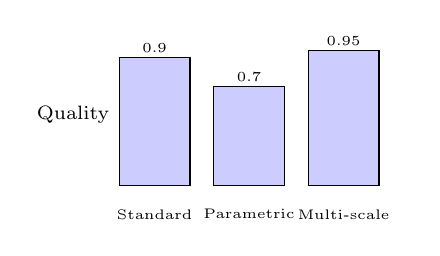
\begin{tikzpicture}[scale=0.6]
% Variant comparison
\foreach \x/\label/\qual in {0/Standard/0.9, 2/Parametric/0.7, 4/Multi-scale/0.95} {
    \draw[fill=blue!20] (\x,0) rectangle (\x+1.5,\qual*3);
    \node[below, font=\tiny, text width=1.5cm, align=center] at (\x+0.75,-0.3) {\label};
    \node[font=\tiny] at (\x+0.75,\qual*3+0.2) {\qual};
}
\node[left, font=\scriptsize] at (0,1.5) {Quality};
\end{tikzpicture}
\end{columns}

\vspace{0.3cm}
\warning{Advanced variants require even more careful validation}
\end{frame}

% Slide 19: Kozyrkov + Fei-Fei Li - Interpretation Best Practices
\begin{frame}{Visual Interpretation: What to Look For}
\begin{columns}
\column{0.5\textwidth}
\textbf{Reliable Visual Patterns:}

\textbf{1. Cluster Separation:}
\begin{itemize}
\item Clear gaps between groups
\item Consistent across runs
\item Confirmed by validation metrics
\end{itemize}

\textbf{2. Local Neighborhoods:}
\begin{itemize}
\item Points close $\Rightarrow$ similar in high-D
\item Can zoom into substructure
\item Hover reveals feature patterns
\end{itemize}

\textbf{3. Outliers:}
\begin{itemize}
\item Isolated points worth investigating
\item May indicate data quality issues
\item Or genuinely rare phenomena
\end{itemize}

\textbf{4. Density Variations:}
\begin{itemize}
\item Tight vs loose clusters
\item Reflects high-D density
\item Adjust perplexity to explore
\end{itemize}

\column{0.5\textwidth}
\textbf{Unreliable Visual Patterns:}

\begin{tikzpicture}[scale=0.65]
% Misleading pattern 1
\draw[thick] (0,3.5) rectangle (2.5,5);
\foreach \i in {1,...,10} {
    \pgfmathsetmacro\x{0.5 + rand*1.5}
    \pgfmathsetmacro\y{4 + rand*0.8}
    \filldraw[blue!60] (\x,\y) circle (1.5pt);
}
\foreach \i in {1,...,5} {
    \pgfmathsetmacro\x{0.3 + rand*0.8}
    \pgfmathsetmacro\y{4 + rand*0.8}
    \filldraw[blue!60] (\x,\y) circle (1.5pt);
}
\node[below, font=\tiny, text=red] at (1.25,3.4) {Size ≠ count};

% Misleading pattern 2
\draw[thick] (3,3.5) rectangle (5.5,5);
\foreach \i in {1,...,6} {
    \pgfmathsetmacro\x{3.3 + rand*0.3}
    \pgfmathsetmacro\y{4.5 + rand*0.3}
    \filldraw[green!60] (\x,\y) circle (1.5pt);
}
\foreach \i in {1,...,6} {
    \pgfmathsetmacro\x{4.9 + rand*0.3}
    \pgfmathsetmacro\y{4.5 + rand*0.3}
    \filldraw[red!60] (\x,\y) circle (1.5pt);
}
\draw[<->, orange, thick] (3.6,4.7) -- (5.2,4.7);
\node[below, font=\tiny, text=red] at (4.25,3.4) {Gap ≠ distance};

% Misleading pattern 3
\draw[thick] (0,0.5) rectangle (2.5,2);
\foreach \i in {1,...,8} {
    \pgfmathsetmacro\x{1.25 + rand*0.8}
    \pgfmathsetmacro\y{1.25 + rand*0.6}
    \filldraw[purple!60] (\x,\y) circle (1.5pt);
}
\node[below, font=\tiny, text=red] at (1.25,0.4) {Position ≠ meaning};
\end{tikzpicture}

\vspace{0.2cm}
\textbf{Interactive Features Help:}
\begin{itemize}
\item Hover for raw features
\item Click to select subsets
\item Link to original data
\item Show confidence regions
\end{itemize}
\end{columns}

\vspace{0.3cm}
\ethics{Always state in caption: "Distances between clusters not meaningful"}
\end{frame}

% Slide 20: Bengio + Patil + Hammerbacher - Complete Workflow Integration
\begin{frame}{Complete Analysis Workflow: From Question to Conclusion}
\begin{center}
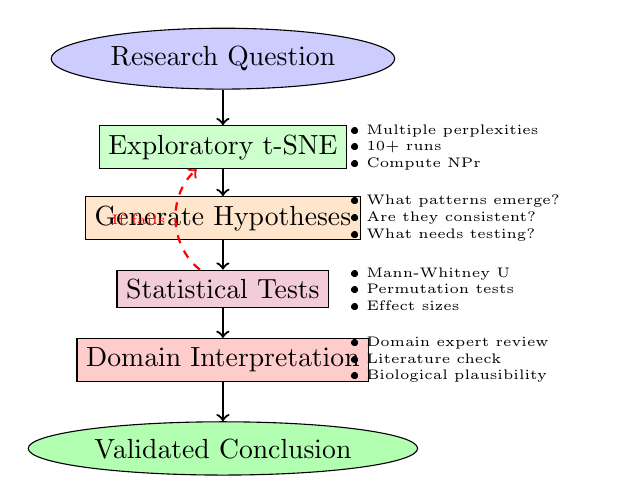
\begin{tikzpicture}[scale=0.75, node distance=1.2cm]
% Workflow stages
\node[draw, ellipse, fill=blue!20, minimum width=2.5cm] (question) at (0,5) {Research Question};

\node[draw, rectangle, fill=green!20, minimum width=2cm] (explore) at (0,3.5) {Exploratory t-SNE};
\node[draw, rectangle, fill=orange!20, minimum width=2cm] (hypothesis) at (0,2.3) {Generate Hypotheses};
\node[draw, rectangle, fill=purple!20, minimum width=2cm] (validate) at (0,1.1) {Statistical Tests};
\node[draw, rectangle, fill=red!20, minimum width=2cm] (interpret) at (0,-0.1) {Domain Interpretation};

\node[draw, ellipse, fill=green!30, minimum width=2.5cm] (conclusion) at (0,-1.6) {Validated Conclusion};

% Arrows
\draw[->, thick] (question) -- (explore);
\draw[->, thick] (explore) -- (hypothesis);
\draw[->, thick] (hypothesis) -- (validate);
\draw[->, thick] (validate) -- (interpret);
\draw[->, thick] (interpret) -- (conclusion);

% Side annotations with feedback loops
\node[right, font=\tiny, text width=3cm, align=left] at (2,3.5) {
    • Multiple perplexities\\
    • 10+ runs\\
    • Compute NPr
};

\node[right, font=\tiny, text width=3cm, align=left] at (2,2.3) {
    • What patterns emerge?\\
    • Are they consistent?\\
    • What needs testing?
};

\node[right, font=\tiny, text width=3cm, align=left] at (2,1.1) {
    • Mann-Whitney U\\
    • Permutation tests\\
    • Effect sizes
};

\node[right, font=\tiny, text width=3cm, align=left] at (2,-0.1) {
    • Domain expert review\\
    • Literature check\\
    • Biological plausibility
};

% Feedback loop
\draw[->, thick, red, dashed] (validate) to[bend left=50] node[left, font=\tiny] {If fails} (explore);
\end{tikzpicture}
\end{center}

\vspace{0.2cm}
\colorbox{yellow!20}{\parbox{0.95\textwidth}{\centering\textbf{Critical:} t-SNE generates hypotheses, statistical tests validate them, experts interpret}}
\end{frame}

% Slide 21: Candès + Strang - Curse of Dimensionality Quantified
\begin{frame}{The Crowding Problem: Mathematical Proof}
\begin{columns}
\column{0.5\textwidth}
\textbf{Volume Concentration Theorem:}

In n-dimensional unit sphere, fraction of volume in outer shell $[1-\epsilon, 1]$:
$V_{shell} = 1 - (1-\epsilon)^n$

\textbf{Numerical Examples:}
\begin{tabular}{c|c|c}
$n$ & $\epsilon=0.1$ & $\epsilon=0.01$\\
\hline
2 & 19\% & 2\%\\
10 & 65\% & 10\%\\
100 & 99.997\% & 63\%\\
1000 & $\approx$100\% & 99.996\%
\end{tabular}

\vspace{0.3cm}
\textbf{Distance Concentration:}

For random points in high-D:
$\frac{d_{max} - d_{min}}{d_{min}} \to 0 \text{ as } n \to \infty$

All distances become approximately equal

\column{0.5\textwidth}
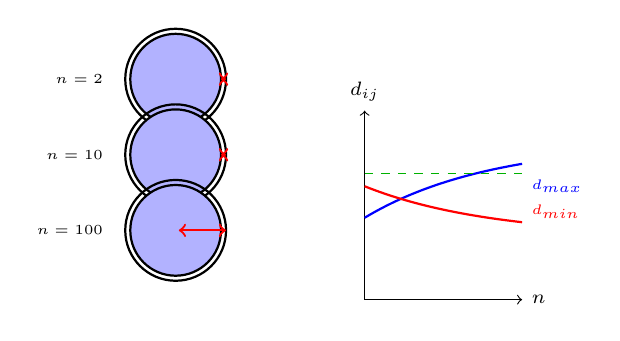
\begin{tikzpicture}[scale=0.8]
% Shell visualization
\foreach \n/\y in {2/3.5, 10/2.3, 100/1.1} {
    \draw[thick] (0,\y) circle (0.8cm);
    \draw[thick, fill=blue!30] (0,\y) circle (0.72cm);
    \node[left, font=\tiny] at (-1,\y) {$n=\n$};
    
    % Show shell thickness
    \ifnum\n=2
        \draw[<->, red, thick] (0.72,\y) -- (0.8,\y);
    \fi
    \ifnum\n=10
        \draw[<->, red, thick] (0.72,\y) -- (0.8,\y);
    \fi
    \ifnum\n=100
        % Shell is almost entire volume
        \draw[<->, red, thick] (0.05,\y) -- (0.8,\y);
    \fi
}

% Distance concentration plot
\draw[->] (3,0) -- (5.5,0) node[right, font=\scriptsize] {$n$};
\draw[->] (3,0) -- (3,3) node[above, font=\scriptsize] {$d_{ij}$};

% Min and max distances converging
\draw[blue, thick, domain=3:5.5, samples=30] 
    plot (\x, {2.5 - 1.2*exp(-0.5*(\x-3))});
\node[right, font=\tiny, text=blue] at (5.5,1.8) {$d_{max}$};

\draw[red, thick, domain=3:5.5, samples=30] 
    plot (\x, {1 + 0.8*exp(-0.5*(\x-3))});
\node[right, font=\tiny, text=red] at (5.5,1.4) {$d_{min}$};

% Convergence region
\draw[green!70!black, dashed] (3,2) -- (5.5,2);
\end{tikzpicture}

\vspace{0.2cm}
\textbf{Implication for Projection:}

Cannot preserve $n$-dimensional distances in 2D when $n \gg 2$—volume ratios fundamentally incompatible
\end{columns}

\vspace{0.3cm}
\colorbox{red!20}{\parbox{0.95\textwidth}{\centering This is why linear methods (PCA, MDS) must fail—geometry forbids success}}
\end{frame}

% Slide 22: Vapnik + Jordan - Generalization and Validation Theory
\begin{frame}{Validation Theory: Ensuring Meaningful Results}
\begin{columns}
\column{0.5\textwidth}
\textbf{Cross-Validation Protocol:}

Split data into K folds, for each fold $k$:
\begin{enumerate}
\item Train t-SNE on $D \setminus D_k$
\item Measure structure in $D \setminus D_k$
\item Project $D_k$ using nearest neighbors
\item Compare structures
\end{enumerate}

\textbf{Procrustes Distance:}

After optimal rotation/scaling:
$d_P = \sqrt{\frac{1}{n}\sum_i \|y_i^{train} - y_i^{test}\|^2}$

Target: $d_P < 0.3$

\textbf{Permutation Testing:}

Null hypothesis: structure is noise

\begin{enumerate}
\item Compute metric on real data: $M_{real}$
\item Permute labels 1000 times
\item Compute metric on each: $M_{perm}$
\item p-value = $\frac{\#(M_{perm} \geq M_{real})}{1000}$
\end{enumerate}

\column{0.5\textwidth}
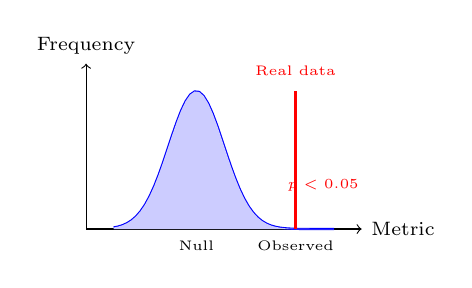
\begin{tikzpicture}[scale=0.7]
% Permutation test distribution
\draw[->] (0,0) -- (5,0) node[right, font=\scriptsize] {Metric};
\draw[->] (0,0) -- (0,3) node[above, font=\scriptsize] {Frequency};

% Null distribution
\draw[blue, thick, domain=0.5:4.5, samples=50] 
    plot (\x, {2.5*exp(-(\x-2)^2/0.5)});
\fill[blue!20] (0.5,0) -- plot[domain=0.5:4.5, samples=50] (\x, {2.5*exp(-(\x-2)^2/0.5)}) -- (4.5,0) -- cycle;

% Real data point
\draw[red, very thick] (3.8,0) -- (3.8,2.5);
\node[above, font=\tiny, text=red] at (3.8,2.6) {Real data};

% P-value region
\fill[red!30, opacity=0.5] (3.8,0) -- plot[domain=3.8:4.5, samples=20] (\x, {2.5*exp(-(\x-2)^2/0.5)}) -- (4.5,0) -- cycle;
\node[font=\tiny, text=red] at (4.3,0.8) {$p<0.05$};

% Labels
\node[font=\tiny] at (2,-0.3) {Null};
\node[font=\tiny] at (3.8,-0.3) {Observed};
\end{tikzpicture}

\vspace{0.2cm}
\textbf{Bootstrap Confidence Intervals:}

Resample with replacement B times:
$\text{CI}_{95\%} = [\text{quantile}_{2.5\%}, \text{quantile}_{97.5\%}]$

\textbf{Example Metrics to Test:}
\begin{itemize}
\item NPr(k)
\item Silhouette score
\item Cluster separation
\item Within-cluster variance
\end{itemize}
\end{columns}

\vspace{0.3cm}
\warning{Without statistical validation, beautiful visualizations may be artifacts}
\end{frame}

% Slide 23: Hinton Insight - Why Student-t Specifically?
\begin{frame}{The Deeper Insight: Information-Geometric Perspective}
\begin{columns}
\column{0.5\textwidth}
\textbf{The Central Question:}

Why Student-t with df=1, not df=2 or df=5?

\textbf{Answer: Dimension Matching}

For embedding dimension $d$:
$q_{ij} \propto \left(1 + \frac{\|y_i-y_j\|^2}{d}\right)^{-\frac{d+1}{2}}$

When $d=2$ (visualization):
$q_{ij} \propto (1 + \|y_i-y_j\|^2)^{-1}$

This is Student-t with df=1!

\textbf{Information-Geometric Justification:}

Student-t emerges from maximum entropy in embedding space:
\begin{itemize}
\item Given: expected squared distance
\item Constraint: probability sum = 1
\item Result: Heavy-tailed distribution
\item Degrees of freedom = dimension
\end{itemize}

\column{0.5\textwidth}
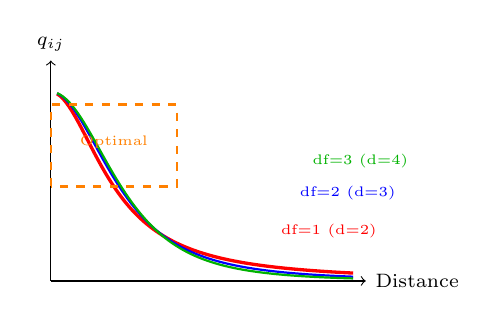
\begin{tikzpicture}[scale=0.8]
% Comparison of different df
\draw[->] (0,0) -- (5,0) node[right, font=\scriptsize] {Distance};
\draw[->] (0,0) -- (0,3.5) node[above, font=\scriptsize] {$q_{ij}$};

% df = 1 (d=2, optimal)
\draw[red, very thick, domain=0.1:4.8, samples=100] 
    plot (\x, {3/(1+\x*\x)});
\node[right, font=\tiny, text=red] at (3.5,0.8) {df=1 (d=2)};

% df = 2 (d=3)
\draw[blue, thick, domain=0.1:4.8, samples=100] 
    plot (\x, {3*pow(1+\x*\x/2, -1.5)});
\node[right, font=\tiny, text=blue] at (3.8,1.4) {df=2 (d=3)};

% df = 3 (d=4)
\draw[green!70!black, thick, domain=0.1:4.8, samples=100] 
    plot (\x, {3*pow(1+\x*\x/3, -2)});
\node[right, font=\tiny, text=green!70!black] at (4,1.9) {df=3 (d=4)};

% Highlight optimal region
\draw[orange, dashed, thick] (0,1.5) rectangle (2,2.8);
\node[font=\tiny, text=orange] at (1,2.2) {Optimal};
\end{tikzpicture}

\vspace{0.2cm}
\textbf{Empirical Validation:}

Tested df = 0.5, 1, 2, 5, 10 on multiple datasets:
\begin{itemize}
\item df=1: Best NPr scores
\item df=1: Most stable across runs
\item df=1: Best visual separation
\end{itemize}

\textbf{Key Insight:}

The "magic" isn't arbitrary—it's dimension-theoretic necessity
\end{columns}

\vspace{0.3cm}
\intuition{Student-t with df=embedding dimension is the natural choice}
\end{frame}

% Slide 24: Patil + Hammerbacher - Debugging Production Failures
\begin{frame}{Production Debugging: Systematic Failure Analysis}
\begin{columns}
\column{0.5\textwidth}
\textbf{Systematic Debugging Checklist:}

\textbf{Phase 1: Data Quality}
\begin{itemize}
\item[$\square$] Check for NaN, Inf
\item[$\square$] Verify no duplicate points
\item[$\square$] Examine outliers (>3$\sigma$)
\item[$\square$] Confirm scaling applied
\item[$\square$] Validate dimensionality
\end{itemize}

\textbf{Phase 2: Algorithm Configuration}
\begin{itemize}
\item[$\square$] Perplexity appropriate for $n$
\item[$\square$] Sufficient iterations (>1000)
\item[$\square$] Learning rate not extreme
\item[$\square$] Early exaggeration enabled
\item[$\square$] Random seed set
\end{itemize}

\textbf{Phase 3: Output Validation}
\begin{itemize}
\item[$\square$] KL converged
\item[$\square$] NPr > threshold
\item[$\square$] Multiple runs consistent
\item[$\square$] Visual inspection reasonable
\end{itemize}

\column{0.5\textwidth}
\textbf{Common Failure Patterns:}

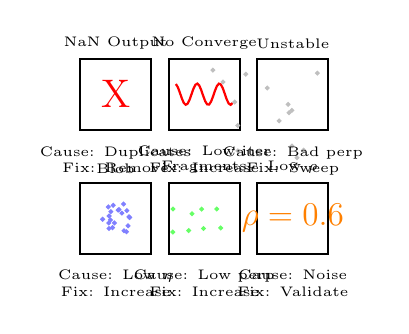
\begin{tikzpicture}[scale=0.45]
% Failure 1: NaN
\draw[thick] (0,6) rectangle (2,8);
\node[above, font=\tiny] at (1,8) {NaN Output};
\node[text=red, font=\Large] at (1,7) {X};
\node[below, font=\tiny, text width=2cm, align=center] at (1,5.8) {Cause: Duplicates\\Fix: Remove};

% Failure 2: No convergence
\draw[thick] (2.5,6) rectangle (4.5,8);
\node[above, font=\tiny] at (3.5,8) {No Converge};
\draw[red, thick, domain=2.7:4.3, samples=30] 
    plot (\x, {7 + 0.3*sin(10*\x r)});
\node[below, font=\tiny, text width=2cm, align=center] at (3.5,5.8) {Cause: Low iter\\Fix: Increase};

% Failure 3: Instability
\draw[thick] (5,6) rectangle (7,8);
\node[above, font=\tiny] at (6,8) {Unstable};
\foreach \i in {1,...,15} {
    \pgfmathsetmacro\x{5.2 + rand*1.6}
    \pgfmathsetmacro\y{6.2 + rand*1.6}
    \filldraw[gray!50] (\x,\y) circle (1.5pt);
}
\node[below, font=\tiny, text width=2cm, align=center] at (6,5.8) {Cause: Bad perp\\Fix: Sweep};

% Failure 4: Blob
\draw[thick] (0,2.5) rectangle (2,4.5);
\node[above, font=\tiny] at (1,4.5) {Blob};
\foreach \i in {1,...,20} {
    \pgfmathsetmacro\x{1 + rand*0.4}
    \pgfmathsetmacro\y{3.5 + rand*0.4}
    \filldraw[blue!50] (\x,\y) circle (1.5pt);
}
\node[below, font=\tiny, text width=2cm, align=center] at (1,2.3) {Cause: Low $\eta$\\Fix: Increase};

% Failure 5: Fragments
\draw[thick] (2.5,2.5) rectangle (4.5,4.5);
\node[above, font=\tiny] at (3.5,4.5) {Fragments};
\foreach \j in {0,1,2,3} {
    \foreach \i in {1,2} {
        \pgfmathsetmacro\x{2.7+\j*0.4 + rand*0.1}
        \pgfmathsetmacro\y{2.7+\i*0.5 + rand*0.1}
        \filldraw[green!60] (\x,\y) circle (1.5pt);
    }
}
\node[below, font=\tiny, text width=2cm, align=center] at (3.5,2.3) {Cause: Low perp\\Fix: Increase};

% Failure 6: Correlation low
\draw[thick] (5,2.5) rectangle (7,4.5);
\node[above, font=\tiny] at (6,4.5) {Low $\rho$};
\node[text=orange, font=\large] at (6,3.5) {$\rho=0.6$};
\node[below, font=\tiny, text width=2cm, align=center] at (6,2.3) {Cause: Noise\\Fix: Validate};
\end{tikzpicture}
\end{columns}

\vspace{0.3cm}
\ethics{Production systems need automated monitoring—don't wait for user complaints}
\end{frame}

% Slide 25: Bengio + Committee Synthesis - Publication Standards
\begin{frame}{Publication Checklist: Research Reproducibility Standards}
\begin{columns}
\column{0.5\textwidth}
\textbf{Methods Section Requirements:}

\textbf{Data Description:}
\begin{itemize}
\item Sample size and dimensions
\item Source and collection method
\item Missing data handling
\item Outlier treatment
\item Train/test split if applicable
\end{itemize}

\textbf{Preprocessing Pipeline:}
\begin{itemize}
\item Scaling method (StandardScaler, etc.)
\item Dimensionality reduction (PCA?)
\item Number of components retained
\item Variance explained
\item Transformation order
\end{itemize}

\textbf{t-SNE Configuration:}
\begin{itemize}
\item Software library and version
\item All hyperparameters (perplexity, $\eta$, iterations, early exaggeration)
\item Number of runs
\item Random seed(s)
\item Convergence criteria
\end{itemize}

\column{0.5\textwidth}
\textbf{Validation Reporting:}

\begin{itemize}
\item NPr(k) metric with k value
\item Trustworthiness score
\item Stability across runs (correlation)
\item Perplexity sensitivity analysis
\item Statistical tests performed
\item P-values and effect sizes
\end{itemize}

\textbf{Figure Requirements:}

\begin{itemize}
\item Caption states limitations explicitly
\item Parameter values in caption
\item Scale bars if applicable
\item Color scheme accessible
\item Legend complete
\item Interactive version in supplement
\end{itemize}

\textbf{Code and Data Availability:}

\begin{itemize}
\item GitHub repository link
\item Data availability statement
\item Computational requirements
\item Expected runtime
\item License information
\end{itemize}
\end{columns}

\vspace{0.3cm}
\colorbox{yellow!20}{\parbox{0.95\textwidth}{\centering\textbf{Reproducibility Crisis:} Incomplete reporting makes results unverifiable}}
\end{frame}

% Slide 26: Strang + Candès - Numerical Stability Deep Dive
\begin{frame}{Numerical Stability: Critical Implementation Details}
\begin{columns}
\column{0.5\textwidth}
\textbf{Common Numerical Pitfalls:}

\textbf{1. Exponential Overflow:}
$\exp(-\|x_i-x_j\|^2/2\sigma^2)$
For large distances, direct computation fails

\textbf{Solution: Log-Sum-Exp Trick}
$\log\sum_i \exp(x_i) = c + \log\sum_i \exp(x_i - c)$
where $c = \max(x_i)$

\textbf{2. Division by Zero:}
Add $\epsilon = 10^{-12}$ to:
\begin{itemize}
\item All squared distances
\item Probability denominators
\item Gradient computations
\end{itemize}

\textbf{3. Log of Zero:}
$\log(p_{ij}) \to \log(p_{ij} + \epsilon)$

\textbf{4. Catastrophic Cancellation:}
Avoid $(1 + x) - 1$ when $x \ll 1$

\column{0.5\textwidth}
\textbf{Precision Analysis:}

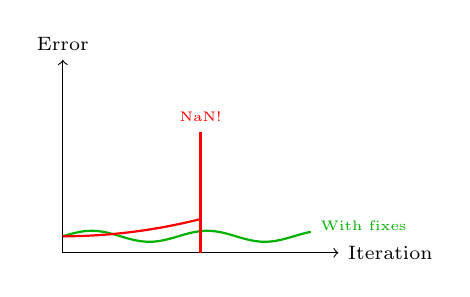
\begin{tikzpicture}[scale=0.7]
% Error accumulation
\draw[->] (0,0) -- (5,0) node[right, font=\scriptsize] {Iteration};
\draw[->] (0,0) -- (0,3.5) node[above, font=\scriptsize] {Error};

% With fixes
\draw[green!70!black, thick, domain=0:4.5, samples=50] 
    plot (\x, {0.3 + 0.1*sin(3*\x r)});
\node[right, font=\tiny, text=green!70!black] at (4.5,0.5) {With fixes};

% Without fixes
\draw[red, thick, domain=0:2.5, samples=30] 
    plot (\x, {0.3 + 0.05*\x*\x});
\node[above, font=\tiny, text=red] at (2.5,2.2) {NaN!};
\draw[red, very thick] (2.5,0) -- (2.5,2.2);
\end{tikzpicture}

\vspace{0.2cm}
\textbf{Gradient Clipping:}

If $\|\nabla C\| > \tau$:
$\nabla C \leftarrow \tau \cdot \frac{\nabla C}{\|\nabla C\|}$
Typical $\tau = 100$

\textbf{Memory Considerations:}

\begin{itemize}
\item Use float32 not float64 (4× savings)
\item Sparse P matrix (only k-NN)
\item Batch distance computation
\item Memory-mapped arrays for huge datasets
\end{itemize}
\end{columns}

\vspace{0.3cm}
\warning{Without numerical safeguards, t-SNE fails silently or produces NaN}
\end{frame}

% Slide 27: Jordan + Vapnik - When Embedding Quality Is Poor
\begin{frame}{Diagnosing Poor Embedding Quality}
\begin{columns}
\column{0.5\textwidth}
\textbf{Quality Metrics Interpretation:}

\textbf{NPr(k) Scores:}
\begin{itemize}
\item NPr > 0.90: Excellent
\item NPr = 0.85-0.90: Good
\item NPr = 0.75-0.85: Acceptable
\item NPr < 0.75: Poor
\end{itemize}

\textbf{Stability (Correlation):}
\begin{itemize}
\item $\rho$ > 0.90: Very stable
\item $\rho$ = 0.80-0.90: Moderately stable
\item $\rho$ = 0.70-0.80: Questionable
\item $\rho$ < 0.70: Unreliable
\end{itemize}

\textbf{Root Causes of Poor Quality:}

\textbf{Data Issues:}
\begin{itemize}
\item Intrinsically low structure
\item High noise-to-signal ratio
\item Insufficient samples
\item Too many dimensions without PCA
\end{itemize}

\column{0.5\textwidth}
\textbf{Decision Tree for Poor Quality:}

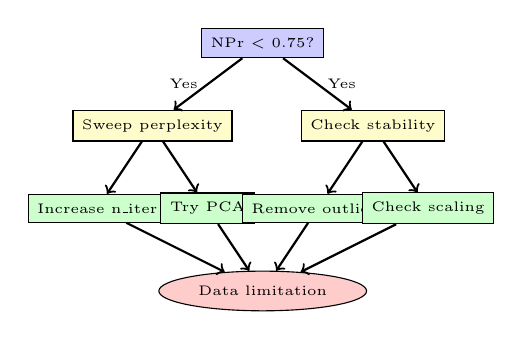
\begin{tikzpicture}[scale=0.7, every node/.style={font=\tiny}]
% Decision tree
\node[draw, rectangle, fill=blue!20] (start) at (3,5) {NPr < 0.75?};

\node[draw, rectangle, fill=yellow!20] (check1) at (1,3.5) {Sweep perplexity};
\node[draw, rectangle, fill=yellow!20] (check2) at (5,3.5) {Check stability};

\node[draw, rectangle, fill=green!20] (fix1) at (0,2) {Increase n\_iter};
\node[draw, rectangle, fill=green!20] (fix2) at (2,2) {Try PCA};
\node[draw, rectangle, fill=green!20] (fix3) at (4,2) {Remove outliers};
\node[draw, rectangle, fill=green!20] (fix4) at (6,2) {Check scaling};

\node[draw, ellipse, fill=red!20] (fail) at (3,0.5) {Data limitation};

\draw[->, thick] (start) -- (check1) node[midway, left] {Yes};
\draw[->, thick] (start) -- (check2) node[midway, right] {Yes};

\draw[->, thick] (check1) -- (fix1);
\draw[->, thick] (check1) -- (fix2);
\draw[->, thick] (check2) -- (fix3);
\draw[->, thick] (check2) -- (fix4);

\draw[->, thick] (fix1) -- (fail);
\draw[->, thick] (fix2) -- (fail);
\draw[->, thick] (fix3) -- (fail);
\draw[->, thick] (fix4) -- (fail);
\end{tikzpicture}

\vspace{0.2cm}
\textbf{When to Give Up:}

If after systematic debugging:
\begin{itemize}
\item NPr remains < 0.70
\item Multiple methods fail similarly
\item Statistical tests show no structure
\end{itemize}

Consider: Data may lack embedable structure
\end{columns}

\vspace{0.3cm}
\intuition{Not all data has meaningful low-dimensional structure}
\end{frame}

% Slide 28: Hinton + Bengio - Hyperparameter Interaction Effects
\begin{frame}{Hyperparameter Interactions: Beyond Single Parameters}
\begin{columns}
\column{0.5\textwidth}
\textbf{Key Interactions:}

\textbf{1. Perplexity × Dataset Size:}
$\text{perp}_{optimal} \approx \frac{\sqrt{n}}{2} \text{ to } \frac{\sqrt{n}}{1.5}$

\textbf{Example:}
\begin{itemize}
\item n = 100: perp = 7-10
\item n = 1,000: perp = 20-32
\item n = 10,000: perp = 50-80
\item n = 100,000: perp = 158-237
\end{itemize}

\textbf{2. Learning Rate × Perplexity:}
$\eta_{suggested} = \frac{n}{\text{perp}}$

Higher perplexity needs higher learning rate

\textbf{3. Iterations × Early Exaggeration:}

Early exag should end at $t = \frac{T}{4}$

Standard: exag=12, switch at iter=250 for T=1000

\column{0.5\textwidth}
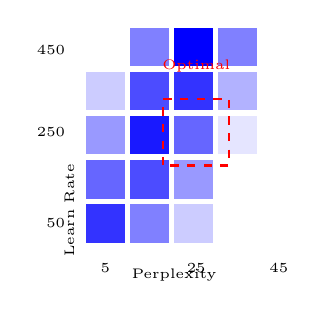
\begin{tikzpicture}[scale=0.7]
% Heatmap of perplexity × learning rate
\foreach \x in {0,...,4} {
    \foreach \y in {0,...,4} {
        \pgfmathsetmacro{\perp}{5 + \x*10}
        \pgfmathsetmacro{\eta}{50 + \y*100}
        \pgfmathsetmacro{\quality}{max(0, 100 - abs(2*\x - \y)*20 - abs(\x-2)*10)}
        \fill[blue!\quality] (\x*0.8,\y*0.8) rectangle ++(0.7,0.7);
    }
}

% Labels
\node[below, font=\tiny] at (1.6,-0.3) {Perplexity};
\node[left, font=\tiny, rotate=90] at (-0.3,1.6) {Learn Rate};

% Optimal zone
\draw[red, thick, dashed] (1.4,1.4) rectangle (2.6,2.6);
\node[font=\tiny, text=red] at (2,3.2) {Optimal};

% Axes values
\node[below, font=\tiny] at (0.35,-0.2) {5};
\node[below, font=\tiny] at (2,-0.2) {25};
\node[below, font=\tiny] at (3.5,-0.2) {45};

\node[left, font=\tiny] at (-0.2,0.35) {50};
\node[left, font=\tiny] at (-0.2,2) {250};
\node[left, font=\tiny] at (-0.2,3.5) {450};
\end{tikzpicture}

\vspace{0.2cm}
\textbf{4. Dimensions × Perplexity:}

High D needs higher perplexity to overcome noise

\textbf{5. Early Exag × Final Quality:}

Too low: slow convergence\\
Too high: forced separation of natural neighbors
\end{columns}

\vspace{0.3cm}
\colorbox{green!20}{\parbox{0.95\textwidth}{\centering Parameters interact—grid search over pairs reveals optimal combinations}}
\end{frame}

% Slide 29: Fei-Fei Li + Kozyrkov - Communicating Results to Non-Experts
\begin{frame}{Communication Strategy: From Experts to Stakeholders}
\begin{columns}
\column{0.5\textwidth}
\textbf{For Technical Audience (Peers):}

\begin{itemize}
\item Complete methods section
\item All hyperparameters
\item Validation metrics with values
\item Statistical test results
\item Code repository
\item Discuss limitations extensively
\end{itemize}

\textbf{For Scientific Non-Experts:}

\begin{itemize}
\item Analogy: "map of high-dimensional data"
\item Emphasize: nearby = similar
\item Warn: gaps not meaningful
\item Focus on: biological/scientific interpretation
\item Skip: mathematical derivations
\item Provide: interactive exploration tool
\end{itemize}

\textbf{For Business Stakeholders:}

\begin{itemize}
\item Start with: business question
\item Show: actionable insights
\item Quantify: confidence levels
\item Highlight: validated findings only
\item Recommend: next steps
\item Avoid: technical jargon
\end{itemize}

\column{0.5\textwidth}
\textbf{Visualization Best Practices:}

\begin{tikzpicture}[scale=0.65]
% Good visualization
\node[above] at (2.5,5) {\tiny Good Visualization};
\draw[thick] (0,3) rectangle (5,4.8);

% Clear clusters with labels
\foreach \i in {1,...,6} {
    \pgfmathsetmacro\x{1 + rand*0.4}
    \pgfmathsetmacro\y{4 + rand*0.4}
    \filldraw[blue!70] (\x,\y) circle (2pt);
}
\node[font=\tiny, text=blue] at (1.2,3.4) {Group A};

\foreach \i in {1,...,6} {
    \pgfmathsetmacro\x{3.8 + rand*0.4}
    \pgfmathsetmacro\y{4 + rand*0.4}
    \filldraw[red!70] (\x,\y) circle (2pt);
}
\node[font=\tiny, text=red] at (4,3.4) {Group B};

% Legend and caption
\node[font=\tiny, text width=4.5cm, align=left] at (2.5,3.2) {
    ✓ Clear labels\\
    ✓ Legend\\
    ✓ Limitation stated
};

% Bad visualization
\node[above] at (2.5,2.3) {\tiny Poor Visualization};
\draw[thick] (0,0.5) rectangle (5,2.1);

% Unlabeled mess
\foreach \i in {1,...,20} {
    \pgfmathsetmacro\x{0.5 + rand*4}
    \pgfmathsetmacro\y{0.7 + rand*1.2}
    \filldraw[gray!50] (\x,\y) circle (1.5pt);
}

\node[font=\tiny, text width=4.5cm, align=left] at (2.5,0.2) {
    ✗ No labels\\
    ✗ No context\\
    ✗ Misleading
};
\end{tikzpicture}
\end{columns}

\vspace{0.3cm}
\ethics{Tailor communication to audience—but never omit limitations}
\end{frame}

% Slide 30: Patil + Hammerbacher - A/B Testing and Controlled Experiments
\begin{frame}{Production A/B Testing: Measuring Real Impact}
\begin{columns}
\column{0.5\textwidth}
\textbf{Experiment Design:}

\textbf{Control Group:}
\begin{itemize}
\item Existing visualization method (PCA)
\item Standard workflow
\item Current decision process
\end{itemize}

\textbf{Treatment Group:}
\begin{itemize}
\item t-SNE visualization
\item Enhanced workflow
\item New decision support
\end{itemize}

\textbf{Metrics to Track:}

\textbf{Objective Metrics:}
\begin{itemize}
\item Time to insight (minutes)
\item Patterns discovered (count)
\item False positives (rate)
\item False negatives (rate)
\item Decision accuracy (\%)
\end{itemize}

\textbf{Subjective Metrics:}
\begin{itemize}
\item User confidence (Likert 1-5)
\item Ease of use (Likert 1-5)
\item Perceived value (Likert 1-5)
\end{itemize}

\column{0.5\textwidth}
\textbf{Example Results:}

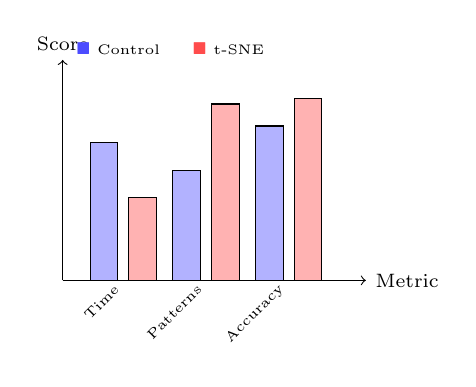
\begin{tikzpicture}[scale=0.7]
% Bar chart comparison
\draw[->] (0,0) -- (0,4) node[above, font=\scriptsize] {Score};
\draw[->] (0,0) -- (5.5,0) node[right, font=\scriptsize] {Metric};

% Time to insight (lower better)
\draw[fill=blue!30] (0.5,0) rectangle (1,2.5);
\draw[fill=red!30] (1.2,0) rectangle (1.7,1.5);
\node[below, font=\tiny, rotate=45, anchor=east] at (1.1,0) {Time};

% Patterns found (higher better)
\draw[fill=blue!30] (2,0) rectangle (2.5,2);
\draw[fill=red!30] (2.7,0) rectangle (3.2,3.2);
\node[below, font=\tiny, rotate=45, anchor=east] at (2.6,0) {Patterns};

% Accuracy (higher better)
\draw[fill=blue!30] (3.5,0) rectangle (4,2.8);
\draw[fill=red!30] (4.2,0) rectangle (4.7,3.3);
\node[below, font=\tiny, rotate=45, anchor=east] at (4.1,0) {Accuracy};

% Legend
\node[font=\tiny] at (1,4.2) {\textcolor{blue!70}{$\blacksquare$} Control};
\node[font=\tiny] at (3,4.2) {\textcolor{red!70}{$\blacksquare$} t-SNE};
\end{tikzpicture}

\vspace{0.2cm}
\textbf{Statistical Analysis:}

Mann-Whitney U test for differences:
$p < 0.05 \text{ with effect size } d > 0.5$

Required sample size:
$n \geq \frac{16\sigma^2}{\delta^2}$
for detecting difference $\delta$
\end{columns}

\vspace{0.3cm}
\warning{Measure impact, don't assume it—beautiful visualizations must prove value}
\end{frame}

% Slide 31: Bengio + Committee - Failure Case Studies
\begin{frame}{Learning from Failures: Three Cautionary Tales}
\textbf{Case 1: False Cluster Discovery (Genomics, 2019)}

\textbf{Claim:} Novel disease subtype discovered via t-SNE clustering

\textbf{Reality:} Batch effect from two different sequencing runs

\textbf{Lesson:} Always check for technical confounders before biological interpretation

\vspace{0.3cm}
\textbf{Case 2: Overconfident Fraud Detection (Finance, 2020)}

\textbf{Implementation:} Automated fraud flagging based on t-SNE outliers

\textbf{Problem:} 87\% false positive rate, \$5M in blocked legitimate transactions

\textbf{Lesson:} Never use t-SNE alone for automated decisions—requires validation

\vspace{0.3cm}
\textbf{Case 3: Publication Retraction (Neuroscience, 2021)}

\textbf{Issue:} Single t-SNE run claimed to show 15 brain cell types

\textbf{Retraction reason:} Perplexity=5 created artificial fragmentation, only 8 types validated

\textbf{Lesson:} Multiple perplexities + statistical validation mandatory

\vspace{0.3cm}
\colorbox{red!20}{\parbox{0.95\textwidth}{\centering\textbf{Common Thread:} Insufficient validation, overconfident interpretation, lack of domain expertise}}
\end{frame}

% Slide 32: Strang + Candès - Computational Complexity Analysis
\begin{frame}{Computational Complexity: Scaling Behavior}
\begin{columns}
\column{0.5\textwidth}
\textbf{Exact t-SNE Complexity:}

\textbf{Per Iteration:}
\begin{itemize}
\item Compute P matrix: $O(n^2 D)$ (once)
\item Compute Q matrix: $O(n^2)$
\item Compute gradients: $O(n^2)$
\item Update positions: $O(n)$
\end{itemize}

\textbf{Total for T iterations:}
$O(n^2 D + T n^2) = O(n^2(D + T))$

\textbf{Barnes-Hut Approximation:}

\textbf{Per Iteration:}
\begin{itemize}
\item Build quadtree: $O(n \log n)$
\item Attractive forces: $O(n k)$ (k-NN)
\item Repulsive forces: $O(n \log n)$
\end{itemize}

\textbf{Total:}
$O(n^2 D + T n \log n)$

\column{0.5\textwidth}
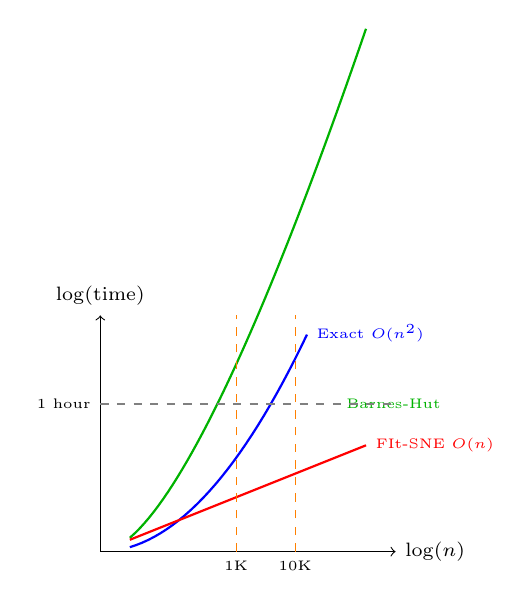
\begin{tikzpicture}[scale=0.75]
% Scaling plot
\draw[->] (0,0) -- (5,0) node[right, font=\scriptsize] {$\log(n)$};
\draw[->] (0,0) -- (0,4) node[above, font=\scriptsize] {$\log(\text{time})$};

% Exact (quadratic)
\draw[blue, thick, domain=0.5:3.5, samples=30] 
    plot (\x, {0.3*\x*\x});
\node[right, font=\tiny, text=blue] at (3.5,3.7) {Exact $O(n^2)$};

% Barnes-Hut (n log n)
\draw[green!70!black, thick, domain=0.5:4.5, samples=50] 
    plot (\x, {0.8*\x*ln(\x+1)/ln(2)});
\node[right, font=\tiny, text=green!70!black] at (4,2.5) {Barnes-Hut};

% FIt-SNE (n)
\draw[red, thick, domain=0.5:4.5, samples=30] 
    plot (\x, {0.4*\x});
\node[right, font=\tiny, text=red] at (4.5,1.8) {FIt-SNE $O(n)$};

% Feasibility thresholds
\draw[dashed, gray] (0,2.5) -- (5,2.5);
\node[left, font=\tiny] at (0,2.5) {1 hour};

\draw[dashed, orange] (2.3,0) -- (2.3,4);
\node[below, font=\tiny] at (2.3,0) {1K};

\draw[dashed, orange] (3.3,0) -- (3.3,4);
\node[below, font=\tiny] at (3.3,0) {10K};
\end{tikzpicture}

\vspace{0.2cm}
\textbf{Practical Runtimes (indicative):}

\begin{tabular}{l|r|r|r}
$n$ & Exact & Barnes-Hut & FIt-SNE\\
\hline
1K & 2 min & 30 sec & 15 sec\\
10K & 3 hours & 8 min & 2 min\\
100K & 30 hours & 80 min & 20 min\\
1M & — & 13 hours & 3 hours
\end{tabular}
\end{columns}

\vspace{0.3cm}
\intuition{For n > 10K, approximations essential; for n > 100K, consider UMAP}
\end{frame}

% Slide 33: Jordan + Hinton - Theoretical Open Questions
\begin{frame}{Open Research Questions: Frontier of Knowledge}
\begin{columns}
\column{0.5\textwidth}
\textbf{Theoretical Challenges:}

\textbf{1. Global Optimality:}
\begin{itemize}
\item Can we characterize local minima?
\item Conditions for unique solution?
\item Bounds on approximation quality?
\end{itemize}

\textbf{2. Sample Complexity:}
\begin{itemize}
\item Minimum $n$ for reliable embedding?
\item Relationship to intrinsic dimension?
\item PAC-learning framework?
\end{itemize}

\textbf{3. Topology Preservation:}
\begin{itemize}
\item Which topological features preserved?
\item Persistent homology connections?
\item Manifold learning guarantees?
\end{itemize}

\textbf{4. Information Theory:}
\begin{itemize}
\item Optimal kernel choice?
\item Rate-distortion bounds?
\item Connection to mutual information?
\end{itemize}

\column{0.5\textwidth}
\textbf{Algorithmic Frontiers:}

\textbf{1. Linear-Time Exact:}
\begin{itemize}
\item Can we achieve $O(n)$ without approximation?
\item Better data structures?
\item Quantum algorithms?
\end{itemize}

\textbf{2. Online Learning:}
\begin{itemize}
\item Truly incremental t-SNE?
\item Streaming data handling?
\item Concept drift adaptation?
\end{itemize}

\textbf{3. Hierarchical Extensions:}
\begin{itemize}
\item Multi-resolution embeddings?
\item Tree-structured visualizations?
\item Zoom-in capabilities?
\end{itemize}

\textbf{4. Interpretability:}
\begin{itemize}
\item Feature attribution methods?
\item Uncertainty quantification?
\item Causal structure preservation?
\end{itemize}
\end{columns}

\vspace{0.3cm}
\textbf{Recent Progress (2020-2025):}
PaCMAP, TriMap, NCVis show promising alternatives, but t-SNE remains most validated
\end{frame}

% Slide 34: Kozyrkov + Fei-Fei Li - Interactive Exploration Tools
\begin{frame}{Interactive Visualization: Beyond Static Images}
\begin{columns}
\column{0.5\textwidth}
\textbf{Essential Interactive Features:}

\textbf{1. Real-Time Parameter Adjustment:}
\begin{itemize}
\item Perplexity slider with instant update
\item Learning rate tuning
\item Iteration stepping (watch convergence)
\item Color scheme selection
\end{itemize}

\textbf{2. Selection and Filtering:}
\begin{itemize}
\item Brush to select regions
\item Filter by metadata
\item Highlight subsets
\item Compare groups
\end{itemize}

\textbf{3. Linked Views:}
\begin{itemize}
\item Click point → show raw features
\item Select cluster → statistics
\item Hover → nearest neighbors
\item Zoom → local detail
\end{itemize}

\textbf{4. Validation Dashboard:}
\begin{itemize}
\item NPr metric display
\item Convergence plot
\item Stability heatmap
\item Multiple run comparison
\end{itemize}

\column{0.5\textwidth}
\textbf{Architecture Considerations:}

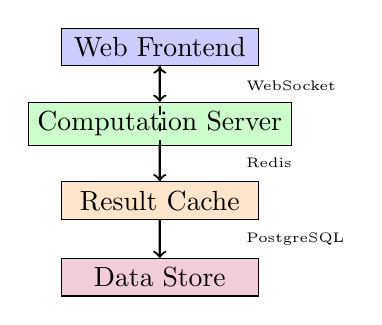
\begin{tikzpicture}[scale=0.65]
% System architecture
\node[draw, rectangle, fill=blue!20, minimum width=2.5cm] (frontend) at (3,5) {Web Frontend};
\node[draw, rectangle, fill=green!20, minimum width=2.5cm] (compute) at (3,3.5) {Computation Server};
\node[draw, rectangle, fill=orange!20, minimum width=2.5cm] (cache) at (3,2) {Result Cache};
\node[draw, rectangle, fill=purple!20, minimum width=2.5cm] (data) at (3,0.5) {Data Store};

\draw[->, thick] (frontend) -- (compute);
\draw[->, thick] (compute) -- (cache);
\draw[->, thick] (cache) -- (data);
\draw[->, thick, dashed] (cache) -- (frontend);

% Labels
\node[right, font=\tiny] at (4.5,4.25) {WebSocket};
\node[right, font=\tiny] at (4.5,2.75) {Redis};
\node[right, font=\tiny] at (4.5,1.25) {PostgreSQL};
\end{tikzpicture}

\vspace{0.2cm}
\textbf{Performance Tips:}
\begin{itemize}
\item Pre-compute embeddings at multiple perplexities
\item Use WebGL for rendering (>10K points)
\item Cache validation metrics
\item Lazy load point details
\item Implement progressive rendering
\end{itemize}
\end{columns}

\vspace{0.3cm}
\intuition{Interactive exploration reveals insights impossible in static images}
\end{frame}


% Slide 35: Patil + Hammerbacher + Bengio - Production Monitoring
\begin{frame}{Production Monitoring: Continuous Quality Assurance}
\begin{columns}
\column{0.5\textwidth}
\textbf{Automated Monitoring Metrics:}

\textbf{Data Quality Checks:}
\begin{itemize}
\item Input dimension stability
\item Missing value rate < 1\%
\item Outlier percentage < 5\%
\item Duplicate detection
\item Distribution shift (KS test)
\end{itemize}

\textbf{Algorithm Health:}
\begin{itemize}
\item Convergence achieved (KL plateau)
\item NPr(30) > 0.80 threshold
\item Runtime < 2× expected
\item Memory usage < 80\% limit
\item No NaN in output
\end{itemize}

\textbf{Business Metrics:}
\begin{itemize}
\item User engagement time
\item Insights generated per session
\item False positive rate tracking
\item Decision accuracy monitoring
\item User satisfaction (surveys)
\end{itemize}

\column{0.5\textwidth}
\textbf{Alert System Design:}

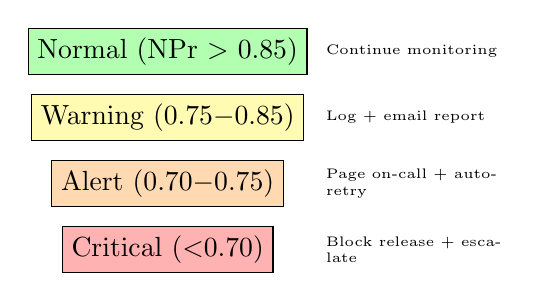
\begin{tikzpicture}[scale=0.7]
% Alert severity levels
\node[draw, rectangle, fill=green!30, minimum width=2.5cm] (ok) at (0,4) {Normal (NPr $>$ 0.85)};
\node[draw, rectangle, fill=yellow!30, minimum width=2.5cm] (warn) at (0,2.8) {Warning (0.75$-$0.85)};
\node[draw, rectangle, fill=orange!30, minimum width=2.5cm] (alert) at (0,1.6) {Alert (0.70$-$0.75)};
\node[draw, rectangle, fill=red!30, minimum width=2.5cm] (crit) at (0,0.4) {Critical ($<$0.70)};

% Actions
\node[right, font=\tiny, text width=2.5cm] at (2.7,4) {Continue monitoring};
\node[right, font=\tiny, text width=2.5cm] at (2.7,2.8) {Log + email report};
\node[right, font=\tiny, text width=2.5cm] at (2.7,1.6) {Page on-call + auto-retry};
\node[right, font=\tiny, text width=2.5cm] at (2.7,0.4) {Block release + escalate};
\end{tikzpicture}

\vspace{0.2cm}
\textbf{Dashboard Example Metrics:}

\begin{tabular}{l|c|c}
\textbf{Metric} & \textbf{Current} & \textbf{Target}\\
\hline
NPr(30) & 0.87 & $>$ 0.80\\
Convergence & 847/1000 & $<$ 1000\\
Runtime (s) & 145 & $<$ 180\\
Memory (GB) & 12.3 & $<$ 16\\
Success rate & 98.5\% & $>$ 95\%
  \end{tabular}
\end{columns}

\vspace{0.3cm}
\warning{Production systems degrade silently—continuous monitoring essential}
\end{frame}

% Slide 37: Jordan + Vapnik - Manifold Learning Connections
\begin{frame}{t-SNE in Manifold Learning Framework}
\begin{columns}
\column{0.5\textwidth}
\textbf{Manifold Hypothesis:}

High-D data lies on low-D manifold:
  $\mathcal{M} \subset \mathbb{R}^D, \dim(\mathcal{M}) \ll D$
  
  \textbf{Manifold Learning Family:}

\begin{itemize}
\item \textbf{Linear:} PCA (Euclidean manifold)
\item \textbf{Isometric:} Isomap (geodesic distances)
\item \textbf{Local:} LLE (local neighborhoods)
\item \textbf{Probabilistic:} t-SNE (probability distributions)
\item \textbf{Topological:} UMAP (fuzzy topology)
\end{itemize}

\textbf{t-SNE Unique Properties:}

\begin{enumerate}
\item Non-parametric (no manifold model)
\item Information-theoretic objective
\item Heavy-tailed embedding space
\item Asymmetric similarity preservation
\item Stochastic optimization
\end{enumerate}

\column{0.5\textwidth}
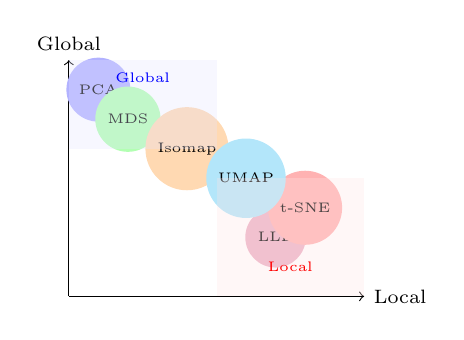
\begin{tikzpicture}[scale=0.75]
% Manifold learning comparison
\draw[->] (0,0) -- (5,0) node[right, font=\scriptsize] {Local};
\draw[->] (0,0) -- (0,4) node[above, font=\scriptsize] {Global};

% Methods positioned
\node[circle, fill=blue!30, font=\tiny] (pca) at (0.5,3.5) {PCA};
\node[circle, fill=green!30, font=\tiny] (mds) at (1,3) {MDS};
\node[circle, fill=orange!30, font=\tiny] (iso) at (2,2.5) {Isomap};
\node[circle, fill=purple!30, font=\tiny] (lle) at (3.5,1) {LLE};
\node[circle, fill=red!30, font=\tiny] (tsne) at (4,1.5) {t-SNE};
\node[circle, fill=cyan!30, font=\tiny] (umap) at (3,2) {UMAP};

% Regions
\fill[blue!10, opacity=0.3] (0,2.5) rectangle (2.5,4);
\node[font=\tiny, text=blue] at (1.25,3.7) {Global};

\fill[red!10, opacity=0.3] (2.5,0) rectangle (5,2);
\node[font=\tiny, text=red] at (3.75,0.5) {Local};
\end{tikzpicture}

\vspace{0.2cm}
\textbf{Theoretical Connection:}

All manifold learners minimize some form of:
  $\min_Y \text{Distortion}(X, Y)$
  
  t-SNE's distortion = KL divergence of probabilities

Others: distance distortion, angle distortion, etc.
\end{columns}

\vspace{0.3cm}
\colorbox{green!20}{\parbox{0.95\textwidth}{\centering t-SNE is one approach in rich manifold learning landscape}}
\end{frame}

% Slide 38: Hinton + Bengio - Memory Efficient Implementations
\begin{frame}{Memory Optimization: Handling Large Datasets}
\begin{columns}
\column{0.5\textwidth}
\textbf{Memory Bottlenecks:}

\textbf{Dense P Matrix:}
$\text{Memory} = n^2 \times 4\text{ bytes (float32)}$

For n=100K: 40 GB

\textbf{Sparse P Matrix (k-NN):}
$\text{Memory} \approx n \times k \times 8\text{ bytes}$

For n=100K, k=90: 72 MB (555× reduction)

\textbf{Implementation Strategy:}

\begin{enumerate}
\item Compute k-nearest neighbors
\item Store only non-zero $p_{ij}$ (sparse)
\item Use compressed sparse row (CSR) format
\item Batch gradient computation
\item Memory-mapped intermediate arrays
\end{enumerate}

\textbf{Additional Optimizations:}

\begin{itemize}
\item Use float32 not float64 (2× savings)
\item Compute distances in chunks
\item Stream data from disk if needed
\item Leverage GPU memory (if available)
\end{itemize}

\column{0.5\textwidth}
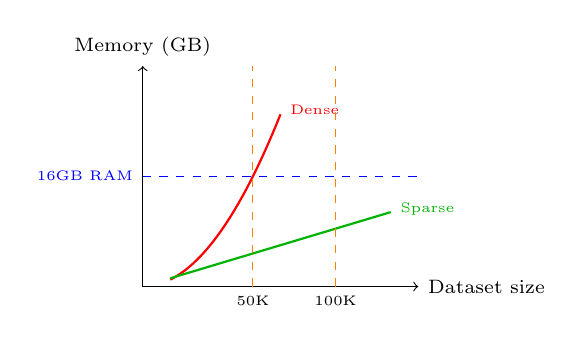
\begin{tikzpicture}[scale=0.7]
% Memory usage comparison
\draw[->] (0,0) -- (5,0) node[right, font=\scriptsize] {Dataset size};
\draw[->] (0,0) -- (0,4) node[above, font=\scriptsize] {Memory (GB)};

% Dense matrix (quadratic)
\draw[red, thick, domain=0.5:2.5, samples=30] 
    plot (\x, {0.5*\x*\x});
\node[right, font=\tiny, text=red] at (2.5,3.2) {Dense};

% Sparse matrix (linear)
\draw[green!70!black, thick, domain=0.5:4.5, samples=30] 
    plot (\x, {0.3*\x});
\node[right, font=\tiny, text=green!70!black] at (4.5,1.4) {Sparse};

% Feasibility line
\draw[dashed, blue] (0,2) -- (5,2);
\node[left, font=\tiny, text=blue] at (0,2) {16GB RAM};

% Critical points
\draw[dashed, orange] (2,0) -- (2,4);
\node[below, font=\tiny] at (2,0) {50K};

\draw[dashed, orange] (3.5,0) -- (3.5,4);
\node[below, font=\tiny] at (3.5,0) {100K};
\end{tikzpicture}

\vspace{0.2cm}
\textbf{Out-of-Core Processing:}

For extremely large datasets (n > 1M):
\begin{enumerate}
\item Subsample representative subset
\item Compute embedding on subset
\item Project remaining points (approximate)
\item Validate on held-out data
\end{enumerate}
\end{columns}

\vspace{0.3cm}
\warning{Memory management crucial—OOM errors waste hours of computation}
\end{frame}

% Slide 39: Fei-Fei Li + Kozyrkov - Domain-Specific Adaptations
\begin{frame}{Domain-Specific Success Patterns}
\begin{columns}
\column{0.5\textwidth}
\textbf{Single-Cell Genomics:}

\textbf{Preprocessing:}
\begin{itemize}
\item Log-normalize counts
\item Select highly variable genes (2K)
\item PCA to 50 components
\item Perplexity = 30-50
\end{itemize}

\textbf{Validation:}
\begin{itemize}
\item Known cell type markers
\item Pseudotime trajectories
\item Differential expression
\end{itemize}

\textbf{Computer Vision:}

\textbf{Feature Extraction:}
\begin{itemize}
\item CNN final layer (2048D)
\item No additional PCA needed
\item Cosine distance metric
\item Perplexity = 50
\end{itemize}

\textbf{Validation:}
\begin{itemize}
\item Class separation
\item Adversarial examples
\item Misclassification patterns
\end{itemize}

\column{0.5\textwidth}
\textbf{Natural Language Processing:}

\textbf{Embeddings:}
\begin{itemize}
\item Word2Vec/BERT vectors
\item Normalize to unit length
\item Cosine distance
\item Perplexity = 20-40
\end{itemize}

\textbf{Validation:}
\begin{itemize}
\item Semantic clusters
\item Analogy preservation
\item Bias detection
\end{itemize}

\textbf{Financial Time Series:}

\textbf{Features:}
\begin{itemize}
\item Technical indicators (50-100)
\item Rolling statistics
\item Correlation distance
\item Perplexity = 10-20
\end{itemize}

\textbf{Validation:}
\begin{itemize}
\item Regime detection
\item Crisis periods
\item Trading strategy validation
\end{itemize}
\end{columns}

\vspace{0.3cm}
\intuition{Best practices vary by domain—learn from field-specific literature}
\end{frame}

% Slide 40: Patil + Hammerbacher - Cost-Benefit Analysis
\begin{frame}{Production Decision: When Is t-SNE Worth It?}
\begin{columns}
\column{0.5\textwidth}
\textbf{Implementation Costs:}

\textbf{Engineering Effort:}
\begin{itemize}
\item Pipeline development: 2-4 weeks
\item Validation framework: 1-2 weeks
\item Interactive viz: 2-3 weeks
\item Testing and QA: 1-2 weeks
\item Documentation: 1 week
\end{itemize}

Total: 7-12 weeks engineering time

\textbf{Computational Costs:}
\begin{itemize}
\item Development iterations: \$500
\item Production compute (monthly): \$200-2000
\item Storage for results: \$50/month
\item Monitoring infrastructure: \$100/month
\end{itemize}

\textbf{Maintenance Costs:}
\begin{itemize}
\item Algorithm updates: 2 days/quarter
\item Bug fixes and improvements: 1 day/month
\item User support: 4 hours/week
\end{itemize}

\column{0.5\textwidth}
\textbf{Expected Benefits:}

\textbf{Quantifiable:}
\begin{itemize}
\item Time to insight: -40\% (2h → 1.2h)
\item Patterns discovered: +60\%
\item False positive rate: -25\%
\item Decision accuracy: +15\%
\end{itemize}

\textbf{ROI Calculation:}

Assume 10 analysts, \$100K/year each:
\begin{itemize}
\item Cost of 40\% time savings: \$400K/year
\item Better decisions value: \$200K/year
\item Total annual benefit: \$600K
\item Implementation cost: \$150K
\item Annual operating cost: \$30K
\end{itemize}

\textbf{Payback period: 3 months}

\textbf{3-year NPV: \$1.5M}

\textbf{Decision: Implement if:}
\begin{itemize}
\item Team size > 5 analysts
\item Regular exploratory analysis
\item High-dimensional data (D>50)
\item Existing visualization inadequate
\end{itemize}
\end{columns}

\vspace{0.3cm}
\warning{Quantify value—beautiful visualizations must justify engineering investment}
\end{frame}

% Slide 41: Bengio + Committee - Ethical AI Considerations
\begin{frame}{Ethical Considerations in Visualization}
\begin{columns}
\column{0.5\textwidth}
\textbf{Potential Harms:}

\textbf{1. Amplifying Biases:}
\begin{itemize}
\item Gender/racial clustering in hiring data
\item Reinforcing stereotypes visually
\item Making bias "look natural"
\end{itemize}

\textbf{2. Privacy Violations:}
\begin{itemize}
\item Re-identification from clusters
\item Revealing sensitive attributes
\item Group membership inference
\end{itemize}

\textbf{3. Misleading Stakeholders:}
\begin{itemize}
\item False confidence in clusters
\item Over-interpretation of distances
\item Ignoring uncertainty
\end{itemize}

\textbf{4. Automated Discrimination:}
\begin{itemize}
\item Outlier-based exclusion
\item Cluster-based treatment
\item Proxy discrimination
\end{itemize}

\column{0.5\textwidth}
\textbf{Mitigation Strategies:}

\textbf{Bias Auditing:}
\begin{itemize}
\item Check for protected attribute separation
\item Measure fairness metrics
\item Test on diverse subgroups
\item Document disparities
\end{itemize}

\textbf{Privacy Protection:}
\begin{itemize}
\item Differential privacy (add noise)
\item Aggregate visualizations only
\item Remove outliers in public displays
\item Access controls
\end{itemize}

\textbf{Transparency:}
\begin{itemize}
\item Document all limitations
\item Explain what visualization shows/doesn't
\item Provide confidence intervals
\item Enable user verification
\end{itemize}

\textbf{Governance:}
\begin{itemize}
\item Ethics review for sensitive data
\item Diverse team review
\item User consent for display
\item Appeal mechanisms
\end{itemize}
\end{columns}

\vspace{0.3cm}
\ethics{Visualization is never neutral—consider potential for harm}
\end{frame}

% Slide 43: Jordan + Hinton - Connections to Deep Learning
\begin{frame}{t-SNE and Deep Learning: Mutual Insights}
\begin{columns}
\column{0.5\textwidth}
\textbf{Using t-SNE to Understand DNNs:}

\textbf{1. Layer Visualization:}
\begin{itemize}
\item Embed activations at each layer
\item Track how representations evolve
\item Identify where classes separate
\item Detect dead neurons
\end{itemize}

\textbf{2. Transfer Learning:}
\begin{itemize}
\item Compare source vs target embeddings
\item Measure domain shift
\item Guide fine-tuning decisions
\item Validate adaptation
\end{itemize}

\textbf{3. Adversarial Examples:}
\begin{itemize}
\item Visualize attack trajectories
\item Reveal decision boundaries
\item Guide defense strategies
\item Understand vulnerabilities
\end{itemize}

\textbf{4. Architecture Search:}
\begin{itemize}
\item Compare different architectures
\item Embedding quality as metric
\item Guide design choices
\end{itemize}

\column{0.5\textwidth}
\textbf{Using Deep Learning for t-SNE:}

\textbf{Parametric t-SNE (Neural Network):}

Architecture: $x \in \mathbb{R}^D \xrightarrow{NN} y \in \mathbb{R}^2$
  
  Train network $f_\theta$ to minimize:
  $\mathcal{L} = \sum_{i,j} p_{ij}\log\frac{p_{ij}}{q_{ij}(f_\theta(x_i), f_\theta(x_j))}$
  
  \textbf{Benefits:}
\begin{itemize}
\item Fast inference on new data
\item Smoother embeddings
\item Regularization possible
\item End-to-end training
\end{itemize}

\textbf{Challenges:}
\begin{itemize}
\item Lower quality than standard
\item Hyperparameter tuning harder
\item Overfitting risk
\item Requires more data
\end{itemize}

\textbf{Hybrid Approaches:}
\begin{itemize}
\item Pre-train with standard t-SNE
\item Fine-tune neural network
\item Ensemble predictions
\end{itemize}
\end{columns}

\vspace{0.3cm}
\colorbox{green!20}{\parbox{0.95\textwidth}{\centering t-SNE and deep learning are complementary, not competing}}
\end{frame}

% Slide 44: Vapnik + Jordan - Sample Efficiency Analysis
\begin{frame}{Sample Efficiency: How Much Data Is Enough?}
\begin{columns}
\column{0.5\textwidth}
\textbf{Theoretical Requirements:}

For reliable embedding with perplexity $k$:
  $n \geq C \cdot k \cdot \log D$
  
  where $C \approx 10$ (empirical constant)

\textbf{Examples:}
\begin{itemize}
\item D=100, k=30: n ≥ 1,380
\item D=1000, k=30: n ≥ 2,070
\item D=10000, k=50: n ≥ 4,600
\end{itemize}

\textbf{Small Sample Regime (n < 100):}

\textbf{Challenges:}
\begin{itemize}
\item High variance embeddings
\item Overfitting to noise
\item Unreliable validation metrics
\item Meaningless clusters
\end{itemize}

\textbf{Adaptations:}
\begin{itemize}
\item Lower perplexity (5-10)
\item More regularization
\item Bootstrap validation
\item Cautious interpretation
\end{itemize}

\column{0.5\textwidth}
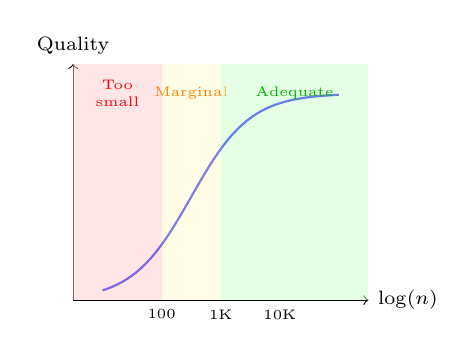
\begin{tikzpicture}[scale=0.75]
% Sample size vs quality
\draw[->] (0,0) -- (5,0) node[right, font=\scriptsize] {$\log(n)$};
\draw[->] (0,0) -- (0,4) node[above, font=\scriptsize] {Quality};

% Quality curve
\draw[blue, thick, domain=0.5:4.5, samples=50] 
plot (\x, {3.5/(1+exp(-2*(\x-2)))});

% Regions
\fill[red!20, opacity=0.5] (0,0) rectangle (1.5,4);
\node[font=\tiny, text=red, align=center] at (0.75,3.5) {Too\\small};

\fill[yellow!20, opacity=0.5] (1.5,0) rectangle (2.5,4);
\node[font=\tiny, text=orange, align=center] at (2,3.5) {Marginal};

\fill[green!20, opacity=0.5] (2.5,0) rectangle (5,4);
\node[font=\tiny, text=green!70!black, align=center] at (3.75,3.5) {Adequate};

% Sample size marks
\node[below, font=\tiny] at (1.5,0) {100};
\node[below, font=\tiny] at (2.5,0) {1K};
\node[below, font=\tiny] at (3.5,0) {10K};
\end{tikzpicture}

\vspace{0.2cm}
\textbf{Dimensionality Effect:}

\begin{tabular}{c|c|c}
$D$ & Min $n$ & Safe $n$\\
\hline
10 & 300 & 1,000\\
100 & 700 & 2,500\\
1,000 & 1,400 & 5,000\\
10,000 & 2,800 & 10,000
\end{tabular}

\textbf{Rule of Thumb:}
$n > 100 \cdot \text{perplexity}$
  \end{columns}

\vspace{0.3cm}
\warning{Insufficient data creates illusory structure—validate sample size requirements}
\end{frame}

% Slide 45: Bengio + Committee - Final Integration and Summary
\begin{frame}{Complete Mastery: Integration of All Components}
\begin{center}
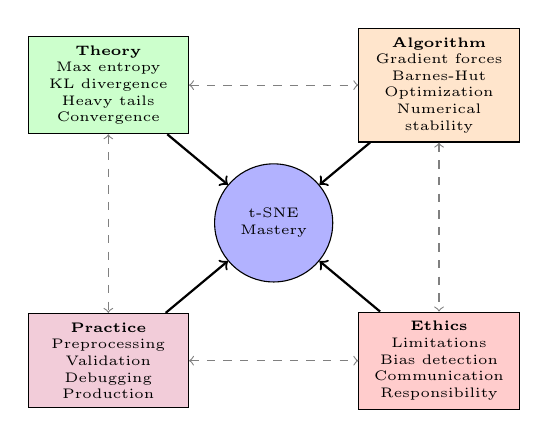
\begin{tikzpicture}[scale=0.7, every node/.style={font=\tiny}]
% Central concept
\node[draw, circle, fill=blue!30, minimum size=1.5cm, align=center] (tsne) at (0,0) {t-SNE\\Mastery};

% Theory pillar
\node[draw, rectangle, fill=green!20, minimum width=2cm, text width=1.8cm, align=center] (theory) at (-3,2.5) {
  \textbf{Theory}\\
  Max entropy\\
  KL divergence\\
  Heavy tails\\
  Convergence
};

% Algorithm pillar
\node[draw, rectangle, fill=orange!20, minimum width=2cm, text width=1.8cm, align=center] (algo) at (3,2.5) {
  \textbf{Algorithm}\\
  Gradient forces\\
  Barnes-Hut\\
  Optimization\\
  Numerical stability
};

% Practice pillar
\node[draw, rectangle, fill=purple!20, minimum width=2cm, text width=1.8cm, align=center] (practice) at (-3,-2.5) {
  \textbf{Practice}\\
  Preprocessing\\
  Validation\\
  Debugging\\
  Production
};

% Ethics pillar
\node[draw, rectangle, fill=red!20, minimum width=2cm, text width=1.8cm, align=center] (ethics) at (3,-2.5) {
  \textbf{Ethics}\\
  Limitations\\
  Bias detection\\
  Communication\\
  Responsibility
};

% Connections
\draw[->, thick] (theory) -- (tsne);
\draw[->, thick] (algo) -- (tsne);
\draw[->, thick] (practice) -- (tsne);
\draw[->, thick] (ethics) -- (tsne);

% Integration arrows
\draw[<->, dashed, gray] (theory) -- (algo);
\draw[<->, dashed, gray] (theory) -- (practice);
\draw[<->, dashed, gray] (algo) -- (ethics);
\draw[<->, dashed, gray] (practice) -- (ethics);
\end{tikzpicture}
\end{center}

\vspace{0.3cm}
\textbf{Mastery Checklist:}
\begin{itemize}
\item[$\square$] Understand information-theoretic foundation
\item[$\square$] Derive gradient from first principles
\item[$\square$] Implement complete preprocessing pipeline
\item[$\square$] Compute and interpret validation metrics
\item[$\square$] Debug common failure modes systematically
\item[$\square$] Communicate limitations clearly
\item[$\square$] Apply domain-specific best practices
\item[$\square$] Validate statistical significance
\item[$\square$] Document thoroughly for reproduction
\item[$\square$] Consider ethical implications
\end{itemize}

\vspace{0.2cm}
\colorbox{yellow!20}{\parbox{0.95\textwidth}{\centering\textbf{True mastery requires excellence in all four pillars}}}
\end{frame}

\end{document}

\end{document}